% !TeX encoding = UTF-8
% !TeX program  = xelatex

\documentclass[12pt,a4paper,openany]{book} 
\usepackage[typeblock=golden]{stb-titlepage}        

%==== Math setup =====================================================
\usepackage{amsmath}%............................. Advanced math (before fonts)
%\usepackage{amssymb}%............................ AMS Symbol fonts

%==== Font setup =====================================================
\usepackage{iftex}
\usepackage{pdflscape}
\usepackage[export]{adjustbox} 
\ifxetex
    \usepackage{fontspec}
    \usepackage[math-style=TeX,
                bold-style=TeX,
               ]{unicode-math}
    \setmainfont{Cambria}%........................ Unicode fonts  (Win)                
    \setsansfont[Scale=MatchLowercase]{Calibri}
    \setmonofont[Scale=MatchLowercase]{Consolas}
    \setmathfont{Cambria Math}
    \defaultfontfeatures{Ligatures=TeX}
    \let\bm\symbfit
\else
    \usepackage[utf8]{inputenc}%.................. Unicode file format
    \usepackage{textcomp}%........................ Additional text symbols
    \usepackage[T1]{fontenc}%..................... Type 1 outline fonts
    \usepackage{bm}%.............................. Bold math fonts
\fi
\normalfont

%==== Units and numbers ==============================================
\usepackage{gensymb}
\usepackage{siunitx}%............................. Unit, number and angle output
    \sisetup{detect-all = true, detect-family = true}
    \sisetup{output-decimal-marker = {.} ,
             group-separator = {\,},
             number-unit-product = {\,},
             inter-unit-product = \mathord{\cdot},
             exponent-product = \mathord{\times},
             separate-uncertainty = true}
         
%==== Ref's, Bib's and Nomencl =======================================
\usepackage{stb-nomencl}%......................... List of symbols 
\usepackage{stb-nomencl}


    \renewcommand*{\UnitLabel}[1]{~[\,\unit{#1}\,]}
\usepackage{stb-bib}%............................. Bibliography (natbib internally)
    \bibliographystyle{stb-bib-eng-a}
    \renewcommand\bibfont{\small}
    \renewcommand\bibsection{\chapter{\bibname}}

%==== Tables + Graphics + Color =====================================
\usepackage{array, float}%............................... Extended table defs 
    \setlength{\extrarowheight}{2pt}
\usepackage{longtable}%........................... Tables can break over pages
\usepackage{graphicx}%............................ Included graphics
\usepackage[font=small]{caption}%................. Customize captions  
\usepackage[table]{xcolor}%....................... Color setup + colortbl 
    
%==== Extra defs for template ========================================
\makeatletter
%---- TOC entries and case
    \renewcommand\contentsname{Table of contents}
    \renewcommand\listfigurename{List of figures}
    \renewcommand\listtablename{List of tables}
    \renewcommand\bibname{List of references}
    \renewcommand\tableofcontents{\chapter*{\contentsname}\@starttoc{toc}}
    \renewcommand\listoffigures{\chapter*{\listfigurename}\@starttoc{lof}}
    \renewcommand\listoftables{\chapter*{\listtablename}\@starttoc{lot}}

%---- Plagiarism signatures
    \newcommand\tstrut[1][4ex]{\rule{0pt}{#1}}
    \newcommand\tdots[1][5cm]{\makebox[#1]{\dotfill}}

%---- Summary head line
    \newcommand\sumheading{%
        \rowcolor[gray]{.9}%
        \centering\arraybackslash%
        \bfseries\normalsize}

%==== User Defs ======================================================
%
% Please insert user defined commands here
% and NOT in the document itself!
%
%
\usepackage{float}
\usepackage{pdfcomment}
\usepackage{pdfpages}
\usepackage{todonotes} 
\usepackage{wasysym} 
\usepackage{tabularx}
\usepackage{colortbl}
\usepackage[table,xcdraw]{xcolor} 
\usepackage{multirow} 
\usepackage{footnote}
\usepackage{adjustbox}
\usepackage{enumitem}
\usepackage{booktabs}
\usepackage{longtable}
\usepackage{pdflscape} % Use pdflscape for rotating the content properly


\makeatother
\parindent 0px
\usepackage{multirow}

%==== Title Page =====================================================
\title{\textbf{Mechatronics Skripsie Report: Tip-thrust Rotary-wing Aircraft}\\[2ex]
       \large Mechatronic Project 478\\Final Report\\[2ex]}                   
\author{\Large Author: Rayde Krüger\\ 
        \large 24723061 \\[5ex]
        \Large Supervisor: Dr. A Gill}                
\address{Department of Mechanical and Mechatronic Engineering\\
        Stellenbosch University \\
        Private Bag X1, Matieland 7602, South Africa.}
\date{\today}                             
\Copyright{2023}{Stellenbosch University.\\ All rights reserved.}

%==== Main Document ==================================================
\setcounter{secnumdepth}{3}
\setcounter{tocdepth}{2}
\raggedbottom
\begin{document}   

\frontmatter%---------------------------------------------------------                    
\maketitle 
\hypersetup{hidelinks}
\include{chaps-front/chap-plagiarism}
\includepdf[pages=-]{Appendix Documents/2024_Skripsie_AI_Use}
\chapter*{Executive summary}
\vspace*{-1.5cm}
\noindent
\begin{longtable}{|p{\dimexpr \linewidth-2\tabcolsep-2\arrayrulewidth}|}
\hline%------------------------------------------------------------
\sumheading  Title of Project \\
\hline%------------------------------------------------------------
Tip-thurst rotary aircraft \\[1ex]

\hline%------------------------------------------------------------
\sumheading  Objectives \\
\hline%------------------------------------------------------------
 The main objective is to design, build and test a prototype of a tip-thrust rotary aircraft with controllable pitch to create directional thrust. \\[1ex]

\hline%------------------------------------------------------------
\sumheading  What is current practice, and what are its limitations? \\
\hline%------------------------------------------------------------
 Current tip-thrust rotary aircraft either use traditional methods for pitch control, such as a swashplate, or use a fixed pitch rotor with additional methods for propulsion to control direction.  \\[1ex]

\hline%------------------------------------------------------------
\sumheading  What is new in this project? \\
\hline%------------------------------------------------------------
 This project investigates the use of a variation of tip-thrust to control the pitch of the rotor.  \\[1ex]

\hline%------------------------------------------------------------
\sumheading  If the project is successful, how will it make a difference? \\
\hline%------------------------------------------------------------
 The controlling pitch using a variation of thrust will decrease the mechanical complexity of rotary aircraft, removing failure points as well as making then easier to produce, lighter and cheaper. \\[1ex]

\hline%------------------------------------------------------------
\sumheading  What are the risks to the project being a success? Why is it expected to be successful? \\
\hline%------------------------------------------------------------
 There is a risk that the pitch cannot change by a large enough amount or fast enough to allow for directional thrust. This risk is reduced through the correct selection and sizing of the components.\\[1ex]

\hline%------------------------------------------------------------
\sumheading  What contributions have/will other students made/make? \\
\hline%------------------------------------------------------------
 Previous student have studied drones, including the thrust produced by the rotors, which will assist in choosing a propulsion method.\\[1ex]

\hline%------------------------------------------------------------
\sumheading  Which aspects of the project will carry on after completion and why? \\
\hline%------------------------------------------------------------
 The control system and optimization of the design can be made to the proof of concept using the mathematical model. \\[1ex]

\hline%------------------------------------------------------------
\sumheading  What arrangements have been/will be made to expedite continuation? \\
\hline%------------------------------------------------------------
 By documenting the procedure, steps followed, including what each component does and how they interact with each other  as well as a project folder will assist any future further contribution. \\[1ex]

\hline%------------------------------------------------------------
\end{longtable}


% \section*{ECSA Requirements}
\vspace{-5mm} % Adjust this value as needed
\small
% \caption{ECSA Requirements} % Uncomment this line for the table caption
\label{tab:ecsa_requirements}
\begin{longtable}{|c|>{\raggedright\arraybackslash}p{2.4cm}|>{\raggedright\arraybackslash}p{2.2cm}|p{7cm}|} 
\hline
Nr   &    \textbf{ECSA Graduate Attribute (GA)}   &   \textbf{Activity addressing attribute}  &   \textbf{Reasoning} \\ \hline
\endfirsthead % Header for the first page
\hline
Nr   &    \textbf{ECSA Graduate Attribute (GA)}   &   \textbf{Activity addressing attribute}  &   \textbf{Reasoning} \\ \hline
\endhead % Header for subsequent pages
\hline
GA1 & \textbf{Problem-solving}  & \ref{sec: MATLAB_Model}, \ref{sec: design} & The project to create a rotary aircraft with tip-thrust controlled pitch, was broken down systematically using the engineering process. In-depth research into this field was performed, and a mathematical model was created of the system. Using the model, a proof of concept was built that can generate directional thrust. \\ \hline 
GA2 & \textbf{Application of scientific and engineering knowledge} & \ref{sec: MATLAB_Model}, \ref{sec: design}, \ref{sec: Experiment} & To create the mathematical model, an in-depth understanding of fluid mechanics was required. This understanding was used to design the rotors to produce the required lift. This model was then validated by measuring the thrust generated by the proof of concept created.   \\ \hline
GA3 & \textbf{Engineering design} & \ref{sec: design} & The rotors of the aircraft were designed using the mathematical model as a guide. The interfaces between all the components required careful designing as well. To control the aircraft, a circuit was designed to detect pitch and speed, send data wirelessly, control the aircraft, and power the components.   \\ \hline
GA4 & \textbf{Engineering methods, skills and tools, including Information Technology} & \ref{sec: MATLAB_Model}, \ref{sec: Software}, \ref{sec: data_Analysis} & The engineering process guided this project, requiring skills such as technical design, critical thinking, and data analysis to achieve the objectives. Software such as MATLAB was used for data processing as well as creating the Blade Element Analysis program. Software such as Excel was used for managing the budget and the pin-out table for the microcontroller and tracker to validate the sensors. \\ \hline
GA5 & \textbf{Professional and technical communication} & \ref{sec: MATLAB_Model} & Many complex topics were discussed during the creation of the mathematical model. This was done concisely, and each step was explained thoroughly to ensure the reader understands the principles the model is based on. \\ \hline
GA6 & \textbf{Individual, team, and multi-disciplinary working} & \ref{sec: design}, Appendix~\ref{sec: Risk_and_saftey} & Throughout the build process, the student worked with technicians to help build the system as well as organizing to have a lab partner at all times for safety. During the project, the student made many large decisions independently of the supervisor. While the guidance provided was insightful, the student was responsible for the research done, designs made, and proof of concept created. \\ \hline
GA7 & \textbf{Independent learning ability} & \ref{sec: Literature_review}, \ref{sec: MATLAB_Model} & As the student is a Mechatronic engineer, advanced fluid mechanics, such as rotor design, blade element analysis, and actuator disc theory, were vital to understanding the behavior of the system. These concepts had to be studied to ensure a firm understanding of the principle, assumptions, and results before creating the mathematical model.\\ \hline
\end{longtable}
\normalsize

%While creating the mathematical model,creative solutions were required to ensurean accurate model was created. To keepwithin budget, some components
\chapter*{Acknowledgements}
    I would like to say thank you to Dr. A. Gill for assisting me to develop this concept to propose as well as for his guidance throughout the project. The insight and encouragement provided was invaluable to this project. I would also like to thank the laboratory engineers and technicians especially as Mr.~K.~Neaves and Mr. F. Zietsman for their assistance while designing and for manufacturing the components of the proof of concept.


\tableofcontents
\listoftables
\listoffigures
\chapter{List of symbols}
% Use stb-nomenclature + siunitx

\begin{Nomencl}[1cm]
\NomGroup{Constants}%-----------------------------------------------
    \item[$\rho = $] air density \qty{1.225}{kg/m\(^3\)}

\NomGroup{Variables}%-----------------------------------------------
    \item[$C_L$]                \UnitLine{Coefficient of lift}{~}
    \item[$C_{L_0}$]            \UnitLine{Lift coefficient offset}{~}
    \item[$C_{L_\alpha}$]       \UnitLine{Lift coefficient gradient}{~}
    \item[$C_D$]                \UnitLine{Coefficient of drag}{~}
    \item[\(V_0\)]              \UnitLine{Axial component of air flow velocity}{m/s} 
    \item[\(V_0\)]              \UnitLine{Axial component of air flow velocity at disk}{m/s} 
    \item[\(V_1\)]              \UnitLine{Resultant flow velocity}{m/s} 
    \item[\(V_2\)]              \UnitLine{Radial component of air flow velocity}{m/s} 
    \item[\(V_\infty\)]         \UnitLine{Free-stream velocity}{m/s}
    \item[\(V_{\omega}\)]       \UnitLine{Far wake velocity}{m/s}        
    \item[$\alpha$]             \UnitLine{Angle of attack}{Deg}
    \item[\(\theta\)]           \UnitLine{Pitch}{rad}
    \item[\(\phi\)]             \UnitLine{Angle made from thrust and lift}{Deg}      
    \item[\(R\)]                \UnitLine{Blade length}{m}    
    \item[\(c\)]                \UnitLine{Blade chord}{m}
    \item[\(T\)]                \UnitLine{Thrust}{N}
    \item[\(Q\)]                \UnitLine{Torque}{N.m}
    \item[\(L\)]                \UnitLine{Drag}{N}
    \item[\(b\)]                \UnitLine{Tip loss coefficient}{~}
    \item[\(C_T\)]              \UnitLine{Thrust coefficient}{~}
    \item[\(B\)]                \UnitLine{Number of blades}{~}
    \item[\(\omega\)]           \UnitLine{Angular velocity}{rads/s}
    \item[\(A\)]                \UnitLine{Area}{m^2}
    \item[\(\zeta \)]           \UnitLine{Damping ratio}{~}
    \item[\(I\)]                \UnitLine{Current}{A}\\

% \NomGroup{Vectors and Tensors}%-------------------------------------
%     \item[$\overrightarrow{\bm{v}}$] Physical vector, see equation ...
\NomGroup{Subscripts}%----------------------------------------------
    \item[$rotor$]          Rotor
    \item[$Prop$]           Propeller
    \item[$motor$]          Tip-thrust/TORB brushless motors
    \item[$n$]              Natural frequency  

\end{Nomencl}

\begin{Nomencl}[1cm]
\NomGroup{Abbreviations}%-----------------------------------------------
    \item[AOA] Angle of Attack
    \item[ESC] Electronic Speed Controller
    \item[FFT] Fast Fourier transform
    \item[PWM] Pulse Width Modulation
    \item[TORB] Thrust On Rotor Blade
    \item[VTOL] Vertical Take-off and Landing
\end{Nomencl}

\mainmatter%----------------------------------------------------------
\numberwithin{figure}{chapter}
\numberwithin{table}{chapter}
\chapter{Introduction}

\section{Background}

    Helicopters are said to be the only aircraft that, since its conception, has saved more lives than they have taken. Their  high level of mobility, vertical take off and landings and their ability to hover give helicopters great versatility. Helicopters are the most common example of a rotary aircraft and are used in environments ranging from rocky, mountainous to stormy seas. With such high stakes it is vital to minimize points of potential failure. One of these failure points is the helicopter's tail rotor. It is required to counter the toque produced by the engine which rotates the main rotor to produce lift. If the tail rotor were to stop working, the helicopter would lose its controllability and would have to land immediately. A jet-tipped rotary aircraft places the propulsion on the tips of the aircraft's rotor and thus does not produce any toque that needs to be canceled, eliminating the need of a tail rotor. As the tail rotor is connected to the same engine that operates the rotor, transmission of the rotation to the tail rotor increases complexity of the helicopter.
     
    \vspace{3mm}
    This project will research, design, construct and test a jet-tipped rotary aircraft which will actuate the pitch of the rotor  the use of propulsion situated at the tip of the blades. Traditional rotary wing aircraft change the rotor's pitch for portions of its rotation, this creates an unbalanced, causing the aircraft to move in the desired direction. Different methods for directional thrust will investigate varying from traditional methods to using the propulsion force itself to control the direction of the aircraft. 
    \vspace*{3mm}
    
    This project, which is prepared for Mechanical Project 448 and prepared by Mr RA Krüger, was proposed by the student after devising the concept with Dr A Gill. The research and results from this project hopes to further the development of tip-propelled rotary aircraft, which currently is a relatively unresearched field. Stated below include the projects scope, objectives, literature review, motivation and planning of the project are outlined. 

%Starting from the big picture, gradually narrow focus down to this project and where this report fits in. Hello world.

\section{Objectives}

The objectives of the project (in some cases the objectives of the report). If necessary describe limitations to the scope.

\section{Motivation}

Why this specific project/report is worth while.


% \chapter{Objectives}

\section{Scope and limitations}
    As previously mentioned this project aims to research, design, build and test a tip-propelled rotary aircraft. The tip-propulsion should vary the pitch of the rotor such that at lower propulsion, the pitch will have a higher pitch, there by increasing the lift generated. As propulsion is increased, the pitch lessens, decreasing the lift produced, but also decreasing the drag generated by the rotor. The final design should prove controllability, but does not need to achieve sustained flight, and thus showing that the aircraft can produce lift in the desired direction will suffice. While a basic understanding of rotor design can be applied to the aircraft's main rotor, it is not the focus of the project and thus no computational fluid dynamics are required either. 

\section{Objectives}
    The objectives of this project are as follows:
    \begin{enumerate}
        \item Construct a working prototype of the created design 
        \item Implement a method to produce directional thrust
        \item Implement a control system for the tip-propulsion
        \item Test and analyse the prototype
    \end{enumerate}
\section{Research questions}
    \subsection{Can the aircraft be fully controlled using the tip propulsion alone?}
    \subsection{What is the efficiency of the aircraft?}
    \subsection{How much thrust can the aircraft produce?}
    \subsection{Which control system method works best?}
    \subsection{How stable is the system?}
    
\section{Motivation}
    As previously mentioned, tip-propelled rotary aircraft remove the need for a tail rotor as they do not produce a torque which needs to be canceled. Traditional shaft-drive helicopters need an engine-to-rotor power transmission to the main rotor and  tail rotor. The output shaft goes into a high rpm/ low torque gearbox and converts the input to low rpm/ high torque output to drive the rotor. 
% \chapter{Literature Review}
\label{sec: Literature_review}
\section{Introduction}
    A rotary-wing aircraft is defined as a configuration in which during take-off and landing, the aircraft derives its lift force directly from an open airscrew, where an airscrew is any actuator disc that has air as its working fluid. These types of aircraft can hover and have Vertical Take-Off and Landing (VTOL) capabilities. Rotary aircraft's airscrews have been given the name of `Rotor' and are characterized by a low disc loading. Disc loading is defined as the average change in pressure across an airscrew. For a rotary aircraft, it is the ratio of the rotor disk area to the total weight of the aircraft (\cite{stepniewski1984rotary}). The most common example of a rotary aircraft is a helicopter. Over the years helicopters have evolved and have gone through many concepts. Tip thrust is one of these changes and will be the focus of this literature review. 

\section{Historical Development}
    One of the earliest concepts of a rotary aircraft can be traced back to Leonardo da Vinci, who came up with the idea of a flying machine based on the Archimedes screw. The Archimedes screw can be thought of as the precursor to the airscrews we have today. While Leonardo's design theoretically worked, it would have been too impractical to build a full-sized version, it did, however, inspire people to create vertical flight machines \citep{stepniewski1984rotary}.\\

    The second factor hindering the development of the helicopter was a lack of understanding of basic aerodynamics. Helicopters are inherently unstable and have a tendency to flip over when in forward flight, this was later discovered to be due to an asymmetrical distribution of lift across the rotor. This is caused by the fact that the lift produced is directly proportional to the incoming air speed squared (\(\text{lift}\;\alpha \text{ air speed}^2\)). When in forward flight one side of the rotor will be moving opposite to the direction of airflow and thus its relative air velocity is higher than the rotor moving in the same direction of the incoming air, one side having increased lift and the other a decreased lift, causing the asymmetry of the forces (\cite{anderson2010helicopters}). This was corrected using a swashplate as well as articulating the blade with flapping and feathering hinges.\\
    

    There were two main points that made the helicopter such a difficult task to accomplish. The first was a lack of an efficient power source. Before the combustion engine, the only power source was the steam engine, which would not produce enough thrust for its weight to make it a viable power source. Even with the combustion engine, it was only after World War I when they began using aluminum that a power-to-weight ratio became large enough to sustain flight. (\cite{stepniewski1984rotary})\\
    
    \begin{figure}[H]
        \centering
        \includegraphics[width = 0.6\textwidth]{figs/WNF V4.jpg}
        \caption{WNF 342 V4 (\cite{Linenbaum_2020})}
        \label{fig:WNF_432_V4}
    \end{figure}

    The first concept of a tip-thrust helicopter can be traced back to the start of World War II, developed by a junior engineer at Wiener Neustädter Flugzeugwerke (WNF), Friedrich von Doblhoff. He proposed to place ramjets on the tip of the rotor and after a short-lived proof of concept managed to impress officials, Friedrich obtained the necessary funding for his first Jet-tipped aircraft. In total four prototypes were constructed, namely WNF 342 V1, V2, V3 and V4, with each design improving on the previous. WNF 342 V4, shown in  Figure~\ref{fig:WNF_432_V4}, used a supercharged engine modified as a compressor to provide air to the rotors and to provide thrust at the back with a pusher propeller. The final design noted that using the jet-tip was inefficient and was used for vertical take-off and landings, when in forward flight, the compressor was switched off, and it operated as an autogyro. Autogyros have freely rotating rotors that spin due to the force of incoming air, this in turn generates lift. The WNF 342 V4 
    design used a mechanism similar to a swashplate to control the cyclic pitch of the rotor and used the air pressure, along with torsional springs, to change the collective pitch (these concepts are further explained in Section~\ref{sec:Helicopter_Control}). The development of tip-thrust was stopped when the test facility was taken by the Allied forces, however, Mr. von Doblhoff would go on to work in America and work on compound helicopters, helicopters which are a hybrid between the rotary-wing and fixed-wing aircraft.  

\section{Helicopter Control} \label{sec:Helicopter_Control}
    Helicopter control relies on the pitch of each blade. The change in pitch causes a change in the angle of attack (AOA). The AOA is directly related to the lift coefficient through \[C_L = C_{L{_0}} +C_{L{_\alpha}} \cdot \alpha\] 
    \begin{minipage}{0.45\textwidth}
        \vspace*{-4mm}
        \begin{align*}
            \text{where} \quad
            &\,C_L \text{ is the coefficient of lift}\\
            &\, C_{L{_0}}\text{ is the offset}  \\
            &\,C_{L{_\alpha}}\text{ is the rate of change of \(C_L\) relative to the AOA}\\
            &\,\alpha \text{ is the angle of attack}\\
        \end{align*}
        \end{minipage}\\

    This is illustrated in Figure \ref{fig:Lift_Vs_AOA}(\cite{angleOfAttackFormula}). Thus increasing the angle of attack increases the lift coefficient, which increases the lift produced. This same concept can be applied to the drag coefficient (\(C_D\)) \\
    \begin{figure} [h]
        \centering
        \includegraphics[width = 0.6\textwidth]{figs/Lift_Vs_AOA.png}
        \caption{Lift vs Angle of Attack (\cite{SKYbary})}
        \label{fig:Lift_Vs_AOA}
    \end{figure}

    Helicopters use collective and cyclic control during flight. The collective control adjusts the pitch of all the blades uniformly, this creates more or less lift overall, allowing the helicopter to rise or fall. The cyclic control varies the pitch depending on where the rotor is in its rotation. Traditional helicopters use swashplates to achieve this control.\\
    A swashplate consists of two plates connected with bearings. This allows the top plate to rotate and the bottom plate to remain fixed. The top plate is connected to the edge of each blade of the rotor by a pitch change arm. This allows control over the pitch by varying the height and angle of the swashplate as can be seen in Figure~\ref{fig:Swashplate} (\cite{anderson2010helicopters}.)
    \begin{figure}
        \centering
        \includegraphics[width = 0.6\textwidth]{figs/Swashplate.png}
        \caption{Lift vs Angle of Attack (\cite{anderson2010helicopters})}
        \label{fig:Swashplate}
    \end{figure}

% The objectives of the project (in some cases the objectives of the report). If necessary describe limitations to the scope.

\section{Current State of the Art} \label{sec:Current_design}
    The concept of tip thrust is an unresearched area of development, however, there a still many applications of this technique, all of which have been applied in different ways. The commonality between all the designs is the method used for propulsion. While some methods make use of ramjets or liquid rockets attached to the tip, it was found during the student's investigation that many designs have been built to create thrust by ejecting an operating fluid out of a nozzle at the tip of the rotor blade. The temperature of the operating fluid splits into two subcategories, a cold-cycle and a hot-cycle. Cold-cycles use compressors and utilize compressed air as the operating fluid. Whereas a hot-cycle uses a gas generator that burns a mixture of compressed air and fuel, creating combustion of products (at temperatures greater than 700\(\degree\)C) which are used as the operating fluid \citep{elmahmodi2014propulsion}.\\
   
    NASA designed a very heavy-lift helicopter (VHLH) using the hot-cycle technique. This was designed as a solution to the weight constraints of shaft-drive helicopters. It was designed such that it could lift an XM-1 Main Battle Tank, which has a total weight of 60 tons, shown in Figure~\ref{fig:VHLH}. The helicopter has a fixed pitch rotor, which is used to generate lift, allowing for VTOL. To control the movement of this helicopter, as the pitch is fixed and cannot use conventional methods, a tail fan with a controllable pitch and controllable louvers, which direct the airflow, was installed at the back. Unfortunately, although the concept was very promising, it was never constructed \citep{head1981}.\\
    \begin{figure}[H]
        \centering
        \includegraphics[width = 0.6 \textwidth]{figs/Heavy lift Helicopter.png}
        \caption{VHLF with a XM-1 Main Battle Tank payload}
        \label{fig:VHLH}
    \end{figure}

    The ATRO-X tip-jet helicopter is an example of a fully constructed jet-tipped helicopter that also makes use of a hot-cycle to provide propulsion. The gas generator is situated on top of the rotor and is connected to a flexible tube to the rotor. The operating fluid travels through the hollow rotors to the tips, where the fluid is expelled. This helicopter only has the main rotor, greatly simplifying the complexity of the helicopter, however, a study by \cite{KOLAREVIC2020112} showed that it was not as efficient as a conventional helicopter. This was partly due to the significant pressure drop of the operating fluid in the rotor channels. It was also stated that the efficiency could be increased by making the rotor larger, however this causes a larger pressure drop. To try to rectify this issue a study by \cite{elmahmodi2014propulsion} tried using the centrifugal force of the rotor as a radial compressor and proved the viability of this concept.\\

    The issues that each of the above concepts encountered will be used to guide all designs regarding the current proof of concept. The current designs have provided very useful insight into what concepts work and which have fundamental issues and should be avoided.

\section{Blade Element Theory}
This method is used to predict the performance of a blade, such as a rotor or a propeller as explained by \cite{blade_element_theory_2024}. The method achieves this by dividing the blade into multiple independent sections along the length of the blade as shown in Figure~\ref{fig: blade_segments}. A force balance is applied to each 2D section to obtain the lift and drag as well as the torque and thrust produced over the section. These values can be summed to predict the total thrust and torque produced by the rotor. \\
As this theory considers the 2D segments, it does not take 3D effects into account, such as flow velocities induced on the blade by the shed tip vortex or the radial component created by the angular acceleration due to the rotation of the rotor. This results in the model overpredicting the thrust produced and underpredicting the torque, resulting in a theoretical efficiency that is between 5\% to 10\% larger than the measured efficiency. One of the flow assumptions made is that the flow on the blade is not stalled, which needs to be kept in mind when designing the system.
\begin{figure}
    \centering
    \includegraphics[width =0.8\textwidth]{figs/Blade_Element.png}
    \caption[Segmented blade]{Diagram showing the blade split into segments \citep{blade_element_theory_2024}}
    \label{fig: blade_segments}
\end{figure}

As shown in Figure~\ref{fig: blade_segments}, the blade can be subdivided to make multiple discrete sections. For this analysis, only the axial and angular components, V\(_0\)  and V\(_2\) respectively, as labeled in Figure~\ref{fig: blade_forces}, of the velocity will be used. The induced flow is assumed to be negligible. V\(_1\) is the summation of these two velocities. 

\begin{figure}[h]
    \centering
    \includegraphics[width =0.8\textwidth]{figs/Blade_Forces.png}
    \caption[Forces acting on the 2D section AA]{Forces acting on the 2D section A-A of Figure~\ref{fig: blade_segments} \citep{blade_element_theory_2024}}
    \label{fig: blade_forces}
\end{figure}
Theta, \(\theta\),  shown in Figure~\ref{fig: blade_forces} is the geometric pitch of the blade. The angle created between the flow velocity vector (V\(_1\)) and \(\theta\) creates the angle of attack~(\(\alpha\)). The lift and drag components are normal and parallel, respectively,  to the blade disk and can be calculated, using Eq. \ref{eq: lift_equation} and Eq. \ref{eq: drag_equation}, to find the thrust and torque of the blade. 
\begin{align}
    \Delta L &= C_L \frac{1}{2} \rho V_1^2 c.dR \label{eq: lift_equation}\\
    \Delta D &= C_D \frac{1}{2} \rho V_1^2 c.dR \label{eq: drag_equation}
\end{align} 
\begin{minipage}{0.45\textwidth}
\vspace*{-8mm}
\begin{align*}
    \text{where} \quad
    &C_L \text{ and } C_D \text{ are for a given } \alpha &\notag \\
    &\rho \text{ is the air density} \notag \\
    &c \text{ is the blade chord} \notag
\end{align*}
\end{minipage}
\\

The difference in angle between thrust and lift can be defined as \[\varphi = \theta - \alpha\] and thus thrust and torque can be found as 
\begin{align}
    \Delta T &= \Delta L\cos(\varphi) - \Delta D\sin(\varphi)  \label{eq: thrust}\\
    \frac{\Delta Q}{R} &= \Delta D\cos(\varphi) + \Delta L\sin(\varphi)  \label{eq: torque}
\end{align}
Combining Eq. \ref{eq: lift_equation} and Eq. \ref{eq: drag_equation} with Eq. \ref{eq: thrust} and Eq. \ref{eq: torque} yields
\begin{align}
    \Delta T &=  \frac{1}{2} \rho V_1^2 c (C_L\cos(\varphi) - C_D\sin(\varphi)) B. dR\\
    \Delta D &=  \frac{1}{2} \rho V_1^2 c (C_D\cos(\varphi) + C_L\sin(\varphi) )B.R.dR
\end{align}
\begin{minipage}{0.45\textwidth}
    \vspace*{-8mm}
    \begin{align*}
        \text{where} \quad
        &B  \text{ is the number of blades} 
    \end{align*}
    \end{minipage}

    \section{Momentum Theory}
        \begin{figure}[h]
            \centering
            \includegraphics[width =0.6\textwidth]{figs/Literature Review/Momentum_theory.png}
            \caption{Momentum theory airstream velocities}
            \label{fig: mometum_theory}
        \end{figure}
        Momentum theory simplifies the rotor of the helicopter's rotor by viewing it as a disc that air flows through and energy is imparted on it by the rotor as stated in  \cite{AflredAerodynamicsOfHelicopters}. As shown in Figure~\ref{fig: mometum_theory}, velocity increases from \(V_0\) to \(V_3\), and it is assumed that the air follows the streamlines, indicated in Figure~\ref{fig: mometum_theory}. The naming convention for the velocities apply only to this section, throughout the report \(V_0,V_1,V_2\) will be as defined in Figure~\ref{fig: blade_forces}. From the mass conservation equation, we know that the \(\dot{m} = \rho S_d V\), through the rotor, thus \(\rho_1 S_1 V_1 = \rho_2 S_2 V_2 = \rho_3 S_3 V_3 =  \rho_4 S_4 V_4 = \text{constant} \), therefore the thrust can be given by
        \begin{align}
            T = \rho S_2 V_1(V_4-V_2) \label{eq: thrust_1}
        \end{align}
         Thrust can also be found as the difference of pressure, \(T=S_2(P_2-P_3)\). Applying Bernoulli's equation which states that the static and dynamic pressure at \(P_1\) be equal to that at \(P_2\), similarly for  \(P_3 \text{ and } P_4\), as \(V_2=V_3\).
        \begin{align*}
           P_1 +\frac{1}{2}\rho V_1^2 &= P_2 +\frac{1}{2}\rho V_2^2 \\
           P_3 +\frac{1}{2}\rho V_3^2 &= P_4 +\frac{1}{2}\rho V_4^2 
        \end{align*}
        These can be rearranged to give
        \begin{align}
            P_3 - P_2 &= \frac{1}{2}\rho(V_4^2 - V_1^2) \notag\\
            \Rightarrow  T &= \frac{1}{2}\rho S(V_4^2 - V_1^2) \label{eq: thrust_2}
        \end{align}
        Making Eq.~\ref*{eq: thrust_1} equal to Eq.~\ref*{eq: thrust_2} we get
        \begin{align*}
            \rho S_2 V_0(V_4-V_1) &=\frac{1}{2}\rho S(V_4^2 - V_1^2)
        \end{align*} 
        which simplifies to
        \begin{align}
            \frac{1}{2}(V_4 + V_1) = V_2 = V_3
        \end{align}

        \section{Gyroscopic Procession}
            This is a phenomenon due to the conservation of angular momentum. It occurs when a force is applied to a rotating object. This force changes the direction of the angular momentum vector. Results in the effects of the applied torque are felt 90\(^circ\) from where the force was applied, as seen in Figure~\ref{fig: gyroscope_procession}. This will cause a helicopter pilot to produce more thrust, by increasing the pitch, at a 90\(^\circ\) offset from the direction the pilot wishes to travel in \citep{gyro}.
        \begin{figure}[H]
        \centering
        \includegraphics[width =\textwidth]{figs/Literature Review/Gyroscopic procession.jpg}
        \caption{Gyroscopic procession}
        \label{fig: gyroscope_procession}
\end{figure}
% \chapter{Planned Activities and Risks}
\section{Planned activities}
    This section aims to outline the activities that will be done to ultimately achieve the aim of the project. These activities will be listed in the order of which they will be done. 
    \subsection{Decide on the type of propulsion}
        As has already been mentioned in Section~\ref{sec:Current_design} the common propulsion method used in most tip-propelled aircraft uses compressed air as the working fluid in either a hot or cold cycle. As mentioned in the project's scope, this will not be considered, however using compressed air could be a potential means of propulsion. The other option is to mount electric motors to the tip and make use of propellers to provide the required thrust. The advantages and disadvantages of each will need to be investigated before a final decision can be made. 
    \subsection{Transfer of potential energy to the rotor tips}
        No matter which means of propulsion is chosen, potential energy, in the form of compressed air or electrical energy, needs to be transported to the tips of the rotor. The fact that the rotor is constantly rotating provides a complicated problem that would need to be overcome to create a system in which each tip can have a user-defined amount of thrust at any time. 
    \subsection{Pitch control}
        The method for how the pitch of the blades needs to be decided. Tests can be performed to see how the chosen propulsion method can influence the pitch of the rotor. Aspects such as feathering and flapping of the rotor need to be taken into account to decide on how the pitch of the rotor can be controlled to achieve directional thrust.
    \subsection{Pitch control system}
        As the pitch will be a parameter that can be influenced by the user, a control system will be required to achieve stability and directional thrust. The types of control systems should be investigated here. Determine whether the system can be used with just a PID controller, whether it needs a lag/lead compensator or if state space is a possibility. If possible a mathematical model should be derived for the prototype to aid with the creation of these control systems.
    \subsection{Pitch and rotor position sensing}
        The system needs to be able to detect the position of the rotor to supply the control system with the correct information, this will be needed to implement directional control as the pitch for directional control needs to vary depending on the position of the rotor's revolution. This will need to be fast and accurate as the rotation will need to be high enough to produce lift and the exact position needs to be known so that directional thrust can be in any direction. 
    \subsection{Computations}
        A method for implementing the system controls and receiving the sensor data needs to be decided one. A method for the way the controller receives user inputs and implements the control system needs to be decided on as this could influence the choice of controller. Options like an ESP32 or a Raspberry Pi would be better if the system is required to be wireless, alternatively, a PLC would more reliable and lighter if it did not need to be wireless.
    \subsection{Rotor and aircraft design}
        As mentioned in the scope, an in-depth rotor design is not required, but research into basic rotor design should be done. A rotor should be designed using all the parameters decided from the above activities to ensure it can produce enough lift and that the method of pitch control can be implemented. The interface of the rotor to the rest of the system should also be considered. The rest of the aircraft will be built around the rotor which incorporates the tip thrust and all the components required to implement the control system.
    \subsection{Build the tip propelled rotary aircraft}\label{sec:build}
        The design should be complete and can be constructed. The design should be constructed using the resources in the mechanical department. 
    \subsection{Test the directional thrust}
        The finished design can be placed on the testing rig. The system will be tested by instructing it to move in different directions. The data will be recorded for analysis. 
    \subsection{Evaluation and repetition}\label{sec:Evaluation}
        Using the data retrieved from the previous activity, the aim of the project can be evaluated. This process can be used to gain information about the system and using this information activities \ref{sec:build} (building) to \ref*{sec:Evaluation} (evaluation) can be repeated to optimize the design until the control system, directional thrust, and pitch control has become satisfactory.
    \subsection{Report writing}
        Once the final prototype has been designed, built and tested, the report can be finalized. This will be continuously worked on and updated throughout the planned activities and will be the last activity of the project.  
    \section{Risks}
        \subsection{Safety}
            This project deals with fast-spinning props and live electricity. Caution must be taken when the prototype is switched on and whenever the wires are being handheld. To minimize this risk, when working with the prototype the power source should be disconnected, this will prevent accidental activations as well as electrocution.
        \subsection{Technical Risks}
            These risks pertain to the risk of equipment or component failure. If equipment malfunction or component failure occurs this could cause harm to either the user or the prototype. To minimize this risk, thorough testing of the equipment and components should be done to ensure they are operating how to be expected. Another potential technical risk is whether the thrust and control system would be able to be operated with enough accuracy and speed to allow for directional thrust. This risk can be reduced through the proper design of the system and the correct selection of components. 
        \subsection{Financial Risks}
            Financial risks include going over budget or standing more than expected. This risk can be minimized through proper budget planning to ensure an accurate budget has been created. Minimizing the technical risk, as mentioned previously, will prevent components or equipment from needing to be replaced.\\
        \subsection{Scheduling risk}
            There is a limited amount of time to complete this project and as such there is a very tight schedule. Unexpected delays could have catastrophic effects on the project and could potentially cause it to become incomplete. To prevent this from occurring, a detailed plan should be devised, and the student should follow it as closely as possible.  
        \subsection{Resources risk}
            This risk relates closely to the previous risk, scheduling risk, as a delay in resources can cause a delay in the entire project. Ordering components or sending designs to be created at the workshop should be done in far enough advance such that if there are any unexpected delays, it will not crucially affect the project's schedule. It can also be reduced by choosing components that are readily available and easy to obtain.\\


% \chapter{Project Scheduled Plan and ECSA Requirements }
    \section{End-of-life strategy}
        Engineers need to ensure each of their projects have an end of life strategy to help ensure sustainable development. For this project a prototype will be developed. Before the design will be made, a list of potential items that could be used for the project will be created. This list could include actuators,  power sources, microcontrollers, sensors and building materials. This list will be used during the design phase and a prototype that uses as many items from previous projects will be created, provided it does not affect its performance. While in the design phase, each piece will be created with the intentions of being able to disassembly the prototype. For all items that must be bought and cannot be reused, an active effort will be made to use recyclable materials and in the event of using a  recyclable  material, a disposal plan will be created, stating the precautions and necessary steps that were training to ensure a safe and sustainable development.
\pagebreak

        \section{ECSA Requirements}
        \captionof{table}{ECSA Requirements} % Use \captionof from caption package for captions outside float environments
        \label{tab:ecsa_requirements}
        \hspace{-2cm}
        \begin{tabular}{|c|>{\raggedright}p{3.5cm}|>{\raggedright}p{4cm}|p{8cm}|} \hline
            Nr   &    \textbf{ECSA Graduate Attribute (GA)}   &   \textbf{Activity addressing attribute}  &   \textbf{Reasoning} \\ \hline
            GA1 & \textbf{Problem-solving}  & 4.1.2,4.1.3,4.1.5 &  The planned activities mentioned all have clear objectives and obstacles that need to be overcome to achieve them. These will require creative solutions to achieve the objective. \\ \hline 
            GA2 & \textbf{Application of scientific and engineering knowledge} & 4.1.4, 4.1.5, 4.1.8 & These actives include creating a mathematical model of the system to then create a control system to be implemented. The building and design process will incorporate workshop trainings and learned from practicals  \\ \hline
            GA3 & E\textbf{ngineering design} & 4.1.1, 4.1.7 &   Each of these activities requires the student to create a solution to the problem by designing a part which will integrate into the system as a whole. \\ \hline
            GA4 & \textbf{Engineering methods, skills and tools, including Information Technology} & 4.1.2, 4.1.5, 4.1.6 & These activities all require skills gained throughout the Engineering course to be able to understand the system and to implement the appropriate solution. \\ \hline
            GA5 & \textbf{Professional and technical communication} & 4.1.11 & Professional report writing to explain the results and how the objectives were met will ensure all the student's information has been conveyed correctly. \\ \hline
            GA6 & \textbf{Individual, team and multi-disciplinary working} & 4.1.8, 4.1.10 & Throughout the build process, the student will need to work with technicians to help build the system. Effectively working with the technicians will ensure that the component will be created to the student's specification. The whole project will have the student's demonstrating their individual work. \\ \hline
            GA7 & \textbf{Independent learning ability} & 4.1.1, 4.1.2 &  As the student is a Mechatronic engineer, the more advanced fluid mechanics, such as rotor design, will require self work to research and understand how the rotor can be designed effectively. \\ \hline
        \end{tabular}
       

        
\chapter{Modelling the System on MATLAB} \label{sec: MATLAB_Model}
    To aid in creating the first design, a mathematical model is required to determine the metrics of the system. This allows for rapid testing and optimization of parameters. 
    % For the full MATLAB code please see the online \href{https://github.com/Rayde29/24723061-Kruger-ProjectFile.git}{\textit{Project~File~here}}. 

    \section{Modelling the Rotor}
        To model the rotor, Blade Element Theory analysis was applied as described by \cite{blade_element_theory_2024}. The rotor was divided into segments and the lift and drag for each segment were calculated. This gives the profile of the thrust and torque along the rotor as can be seen in Figure~\ref{fig: thrust_over_radius} and Figure~\ref{fig: torque_over_radius}, respectively. The sum of each segment will result in the total thrust and torque produced by the rotor.
        The thrust and torque produced by each segment is an iterative process as the incoming flow velocity is unknown. In the first iteration, it is assumed to be zero, and thus the angle of attack is equal to the pitch of the rotor. The incoming air can be calculated using the first approximation of thrust and with Newton's First Law:
        \begin{align*}
            F & = ma\\
            T & = \frac{d(mV)}{dt}
        \end{align*}
        Assuming air above the rotor is stationary
        \begin{align*}
            T &= \dot{m}V\\
            T &= \rho V_{disk} A V
        \end{align*} 
        This gives the thrust in terms of the air velocity and velocity at the disk. As stated by momentum theory and by \cite{AflredAerodynamicsOfHelicopters}, the far wake velocity is half that of the air velocity \(V\) at the disk. Thus, for hover, assuming the free stream velocity is zero, the axial velocity at the disk can be given by

        \begin{align*}
            T &= (\rho \pi R^2 V_{disk} )2V_{disk}\\
            V_{disk} &= \sqrt{\frac{T}{2 \rho \pi R^2}}
        \end{align*}
        
        Using this and the angular rotation of the rotor, the angle of attack can be found as \[\alpha = \theta - \arctan\left(\frac{V_{disk}}{\frac{2}{3}R\omega_{Rotor}}\right)\] Two-thirds of the blade's length is used as the speed of the blade is not constant along its radius, so the speed of the centroid was used to try to approximate the average angle of attack along the blade. 
        It was seen that the thrust and torque converge after 25 iterations. Resulting in the profiles as seen in Figure~\ref{fig: thrust_over_radius} and Figure~\ref{fig: torque_over_radius}.


        \begin{figure}[h]
            \centering
            \begin{minipage}{0.45\textwidth}
                \centering
                \includegraphics[width=\textwidth]{figs/Model/Rotor/Thrust_Vs_Radius.png}
                \caption{Thrust predicted over the length of the rotor}
                \label{fig: thrust_over_radius}
            \end{minipage}\hfill
            \begin{minipage}{0.45\textwidth}
                \centering
                \includegraphics[width=\textwidth]{figs/Model/Rotor/Torque_Vs_Radius.png}
                \caption{Torque predicted over the length of the rotor}
                \label{fig: torque_over_radius}
            \end{minipage}
        \end{figure}

        Using 300 segments resulted in predictions that are 0.5\% different from the value obtained using five thousand segments. This was an acceptable value and was used to reduce the computational cost of the model.

        % Using these results, the number of segments can be found which minimizes the computational cost, while having sufficient accuracy. Figure~\ref{fig: segments_vs_prediction} shows the predicted torque and thrust for the number of segments the rotor is split into. It can be seen that both graphs plateau and that after a certain amount of segments, the increase in accuracy is not beneficial for the computational power. The elbow of both of the predictions is around three hundred segments, which results in predictions that are 0.5\% different from the value obtained using five thousand segments. It was decided that it was sufficient accuracy for the computational cost and thus three hundred segments were used for the model.
        % \begin{figure}[h]
        %     \centering
        %     \includegraphics[width=0.6\textwidth]{figs/Model/Rotor/Segments_Vs_Error.png}
        %     \caption{Predicted torque and thrust vs the number of segments}
        %     \label{fig: segments_vs_prediction}
        % \end{figure}
        % \\
        The Blade Element analysis considers the 2D segments and thus does not take 3D effects into account. This results in the model underpredicting the torque and overpredicting the thrust produced. One of the assumptions neglects the tip vortices which will decreased the thrust produced. To compensate for the decreased thrust, the predicted thrust can be multiplied by a tip-loss factor \(b\). \cite{AflredAerodynamicsOfHelicopters} describe the tip-loss factor as a coefficient that is multiplied by the radius of the rotor for the thrust calculations. This assumes that from \(b\times R\) of the rotor, it will produce zero lift but still have drag. It is defined as 
            \begin{align}
                &b = 1 -\frac{\sqrt{2C_T}}{B}
            \end{align}
            \begin{minipage}{0.45\textwidth}
                \vspace*{-8mm}
                \begin{align*}
                    \text{where} \quad
                    &B  \text{ is the number of blades} \\
                    &C_T  \text{ is the rotor thrust coefficient}
                \end{align*}
                \end{minipage}
                \\
                
        The thrust coefficient is the thrust per unit blade span and can be defined as
        \begin{align}
            &C_T= \frac{T}{\pi R^2 \rho (\omega_{Rotor} R).^2}
        \end{align}
        \\
        The above gives the lift profile along each blade of the rotor, but finding the total thrust for different angular velocities is more vital for designing the initial proof of concept. To do this the thrust and torque values were calculated for a range of angular velocities and their values were stored. An exponential function is then fitted onto these equations, as can be seen in Figure~\ref{fig: thrust_vs_angular_velocity} and Figure~\ref{fig: torque_vs_angular_velocity}, resulting in two equations that can be used to predict the amount of thrust and torque produced for a given angular velocity, Eq.~\ref{eq: fitted_thrust} and Eq.~\ref{eq: fitted_torque}, respectively.
        \begin{align}
            T &= 0.01805 \omega_{Rotor} ^2 \label{eq: fitted_thrust}\\
            Q &= 0.002216 \omega_{Rotor} ^2 \label{eq: fitted_torque}
        \end{align}


        \begin{figure}[H]
            \centering
            \begin{minipage}{0.45\textwidth}
                \centering
                \includegraphics[width=0.8\textwidth]{figs/Model/Rotor/Thrust_Vs_Rotor_Angular_Velocity.png}
                \caption[Rotor thrust vs angular velocity]{Thrust predicted vs angular velocities and the fitted exponential equation}
                \label{fig: thrust_vs_angular_velocity}
            \end{minipage}\hfill
            \begin{minipage}{0.45\textwidth}
                \centering
                \includegraphics[width=0.8\textwidth]{figs/Model/Rotor/Torque_Vs_Rotor_Angular_Velocity.png}
                \caption[Rotor torque vs angular velocity]{Torque predicted vs angular velocities and the fitted exponential equation}
                \label{fig: torque_vs_angular_velocity}
            \end{minipage}
        \end{figure}
    \section{Modelling the Propellers}
        Modeling the propellers for the tip thrust used a similar approach as for the rotor except that the propellers are smaller, and the accuracy is not as crucial for designing the proof of concept. The thrust and torque produced were calculated using one section with the radius being two-thirds of the blade length as this was shown to give an accurate value with one section when compared to multiple sections. \\
        The propeller's pitch is described by the distance the propeller moves forward per rotation and thus to find the average angle of the pitch it can be found as \[\theta_{prop} = \arctan\left(\frac{\text{Pitch}}{\pi d}\right)\]
        The incoming airflow of each propeller can be found by multiplying the angular velocity of the rotor by the position along the rotor blade of the propellers. The high velocities of the inflowing air will decrease the angle of attack. This requires the propellers to have high angular velocities to ensure an angle of attack that produces thrust. Choosing a propeller with a high pitch can ensure that the incoming air meets the blade at a more effective angle of attack. 
        \\
        As the incoming air velocity is dependent on the angular velocity, this results in a thrust and torque versus the angular velocity of the propellers to have a different shape depending on the angular velocity. This can be seen in  Figure~\ref{fig: prop_thrust_vs_velocity} and Figure~\ref{fig: prop_torque_vs_velocity}. 

        \begin{figure}[h]
            \centering
            \begin{minipage}{0.45\textwidth}
                \centering
                \includegraphics[width=\textwidth]{figs/Model/Props/Prop_thrust_vs_speed.png}
                \caption[Propeller thrust versus speed graph]{Propeller thrust versus its speed for different values of rotor angular velocity}
                \label{fig: prop_thrust_vs_velocity}
            \end{minipage}\hfill
            \begin{minipage}{0.45\textwidth}
                \centering
                \includegraphics[width=\textwidth]{figs/Model/Props/Prop_torque_vs_speed.png}
                \caption[Propeller torque versus speed graph]{Propeller torque versus its speed for different values of rotor angular velocity}
                \label{fig: prop_torque_vs_velocity}
            \end{minipage}
        \end{figure}
        Each graph for the thrust, however, can be fitted by a parabolic graph, but with different coefficients depending on the rotor's angular velocity. The solution for this was to find a relationship between the coefficients and the rotor's angular velocity. The change of these coefficients can be seen in Figure~\ref{fig: p1_coefficient},\ref{fig: p2_coefficient} and \ref{fig: p3_coefficient}, in which \[T_{prop} = P_1\omega_{prop}^2 + P_2\omega_{prop} +P_3\] 
        
        \begin{figure}[h]
            \centering
            \begin{minipage}{0.31\textwidth}
                \centering
                \includegraphics[width=\textwidth]{figs/Model/Props/P1_Coeffcient.png}
                \caption{Coefficient P1}
                \label{fig: p1_coefficient}
            \end{minipage}\hfill
            \begin{minipage}{0.31\textwidth}
                \centering
                \includegraphics[width=\textwidth]{figs/Model/Props/P2_Coeffcient.png}
                \caption{Coefficient P2}
                \label{fig: p2_coefficient}
            \end{minipage}\hfill
            \begin{minipage}{0.32\textwidth}
                \centering
                \includegraphics[width=0.99\textwidth]{figs/Model/Props/P3_Coeffcient.png}
                \caption{Coefficient P3}
                \label{fig: p3_coefficient}
            \end{minipage}
        \end{figure}
        From these graphs, clear relationships can be seen with all three coefficients and the angular velocity. Fitting curves to each coefficient result in the Eq.~\ref*{eq: prop_thrust}, which fully describes the thrust produced by tip-thrust.
        \begin{align}
            T_{prop}&=
            \left((-2.500\times 10^{-16})\omega_{rotor} ^3 + (1.517\times 10^{-12})\omega_{rotor} ^2 + (-1.314\times 10^{-9})\omega_{rotor} \right.\notag\\
            &\left. + (1.037\times 10^{-6})\right)\omega_{prop}^2 + \left((-7.806\times 10^{-12})\omega_{rotor}^2+(7.144\times 10^{-9})\omega_{rotor}^2 \right. \notag\\
            &\left. + (-1.301\times 10^{-5})\omega_{rotor}  -0.0003 \right)\omega_{prop}+\left( (-4.593\times 10^{-5})\omega_{rotor}^2 \right. \notag\\
            &\left.+ (-1.006\times 10^{-3})\omega_{rotor} +0.2227\right) \label{eq: prop_thrust}
        \end{align}

    \section{Optimization of Tip Thrust Positions}
        As previously mentioned the incoming airflow for the tip thrust is equal to the position of the tip thrust multiplied by the rotor's angular velocity. Having the propulsion at the end of the rotor will maximize the torque produced, however, it will have a higher incoming airflow and require higher rotation from the tip-thrust motors to produce thrust.\\ 
        The optimum point of the tip-thrust motors would be where the thrust required for the torque is minimized, and the thrust produced is maximized. To find the optimum point the rotor angular velocity and tip thrust angular velocity were kept constant at an expected operating value. The thrust produced by the motors as well as the thrust that would be required to produce the torque were calculated for each percentage length along the rotor as seen in Figure~\ref{fig: thrust_req_vs_available}. This took the hub diameter into account, thus at 0\% of the rotor span (i.e. the base of the rotor), the torque does not tend to infinity.

        \begin{figure}[h]
            \centering
            \begin{minipage}{0.45\textwidth}
                \centering
                \includegraphics*[width = \textwidth]{figs/Model/Rotor/Thrust_avaliable_vs_required.png}
                \caption[Thrust available and required for tip-thrust positions]{Thrust available and the thrust required for a position along the rotor}
                \label{fig: thrust_req_vs_available}
            \end{minipage}\hfill
            \begin{minipage}{0.45\textwidth}
                \centering
                \includegraphics*[width =\textwidth]{figs/Model/Rotor/Optimisation_curve.png}
                \caption{Optimization curve}
                \label{fig: optimization_curve}
            \end{minipage}
        \end{figure} 
        The thrust required and thrust available were standardized, so they could be compared. The two standardized sets of values were subtracted from each other and the turning point of the resulting graph was used as the optimized position along the rotor. As can be seen in Figure~\ref{fig: optimization_curve}, this is around 32.5\% along the rotor blade. While this does vary slightly depending on the motor's angular velocity, at the expected velocity a position of 32.5\%  of the rotor is optimum and is close to the mean for the position that incorporates the range of motor speed.\\
  
        As the thrusts will no longer be placed on the tip of the rotors, it was believed that they should be referred to as TORB motors (Thrust On Rotor Blade) from this point forward. This was chosen to give a more accurate name to this method of creating rotational actuation.
    \section{Combined Model}
        Using the models created above, the system can take the amount of thrust required and will output the torque produced and required thrust. 
        \begin{align}
            \omega_{rotor} =& \sqrt{55.4T_{rotor}}\\
            Q_{Rotor} =& 0.1228T_{rotor}
            % T_{prop} = P_1\omega_{prop}^2 + P_2\omega_{prop} +P_3
            % \omega_{prop} = \frac{-\left[(-7.806 \times 10^{-12})\omega_{rotor}^2 + (7.144 \times 10^{-9})\omega_{rotor} - 1.301 \times 10^{-5}\right] + \sqrt{\left[(-7.806 \times 10^{-12})\omega_{rotor}^2 + (7.144 \times 10^{-9})\omega_{rotor} - 1.301 \times 10^{-5}\right]^2 - 4 \left[(-2.500 \times 10^{-16})\omega_{rotor}^3 + (1.517 \times 10^{-12})\omega_{rotor}^2 + (-1.314 \times 10^{-9})\omega_{rotor} + 1.037 \times 10^{-6}\right] \left[(-4.593 \times 10^{-5})\omega_{rotor}^2 + (-1.006 \times 10^{-3})\omega_{rotor} + 0.2227 - T_{prop}\right]}}{2 \left[(-2.500 \times 10^{-16})\omega_{rotor}^3 + (1.517 \times 10^{-12})\omega_{rotor}^2 + (-1.314 \times 10^{-9})\omega_{rotor} + 1.037 \times 10^{-6}\right]}
                        % \quad \Rightarrow \omega_{prop} =& -\left((-1.775\times 10^{-15})\left(\sqrt{161.5T_{Rotor}}\right) ^3 + (3.676\times 10^{-12}) \right. \notag\\
            % &\left.\times\sqrt{161.5T_{Rotor}} ^2  + (-1.974\times 10^{-9})\sqrt{161.5T_{Rotor}}\notag  \right) \pm  \\ 
            % & \left[(-1.775\times 10^{-15})\left(\sqrt{161.5T_{Rotor}}\right) ^3 + (3.676\times 10^{-12})\right] \notag
        \end{align}


        % \todo[color=blue!10]{Do the whole formula}

        
        \section{Pitch Model}
            To estimate the amount of torque required to change the pitch of the rotor a rotational mass-spring-damper model was created. This models the system which assumes there will be natural damping, so no artificial damping will be introduced, and the system will be rotating on a low friction bushing, thus the effects of friction have been neglected. The model assumes a value for the moment of inertia based on a CAD model of the rotor. \\
            Two models have been created, one for a step input to achieve a fixed pitch change and a second one to achieve a varying pitch to create sinusoidal output which can be seen in Figure~\ref{fig: pitch_change}. This will create a differential amount of thrust that will induce forward movement. For these two models, the control of the steady state of the system was the objective, and thus the rise time and overshoot was a lower priority.
            \begin{figure}[h]
                \centering
                \begin{minipage}{0.45\textwidth}
                    \centering
                    \includegraphics*[width =0.9\textwidth]{figs/Model/Pitch/Pitch_variation.jpg}
                    \caption{Pitch change sinusoidally}
                    \label{fig: pitch_change}
                \end{minipage}\hfill
                \begin{minipage}{0.45\textwidth}
                    \centering
                    \includegraphics*[width = 0.5\textwidth]{figs/Model/Pitch/Free_body_diagram_spring.jpg}
                    \caption{Free body diagram of tip thrust }
                    \label{fig: free_body_diagram}
                \end{minipage}
            \end{figure} 
            \subsection{Step Input}
            From Figure~\ref{fig: free_body_diagram}, a differential equation can be derived for a step input to give Eq.~\ref*{eq: step_input_reponse}.
            % \todo[color=green!20]{Put the proper zeta in}
            \begin{align}
                \ddot{\theta} +2\omega_{n}\zeta\dot{\theta} + \omega _{n}^2 \theta &= \frac{M_{required}}{I_{airfoil}} \label{eq: step_input_reponse}
            \end{align}
            As no artificial damping will be added to the system, it was assumed to be an under-damped system and an arbitrary dampening coefficient has been used, and it is assumed it is starting where \(\theta\) and \(\dot{\theta}\) is zero. Using this information, the solution to Eq.~\ref{eq: step_input_reponse} given by Eq.~\ref{eq: step_input_reponse_solution}.
            \begin{align}
                \theta(t) &= Ae^{-\zeta \omega_n t}\sin(\omega_d t +\phi) + \frac{M_{required}}{k} \label{eq: step_input_reponse_solution}
            \end{align}
            \begin{minipage}{0.45\textwidth}
                \vspace*{-4mm}
                \begin{align*}
                    \text{where} \quad
                    &A = \frac{-\frac{M_{required}}{k}}{\sin(\phi)} \\
                    &M_{required} = \theta_{required}k\\
                    &\theta_{required} \text{ is the desired pitch}
                \end{align*}
                \end{minipage}
                \\
                \begin{figure}[h]
                    \centering
                    \includegraphics*[width = 0.65\textwidth]{figs/Model/Pitch/System_response _for _step_input.png}
                    \caption{System response to a step input}
                    \label{fig: step_response}
                \end{figure}
                Figure~\ref{fig: step_response} shows the system response to an applied moment that results in a steady state of 0.0873 rads (5\(^\circ\)). It can be seen that the response from the system has some oscillation, however its settling time is reasonably fast and would suffice for the proof of concept.
                \vspace{-5mm}
            \subsection{Sinusoidal Input}
                For a sinusoidal input the differential equation is given by Eq.~\ref*{eq: cos_input_reponse}
                \begin{align}
                    \ddot{\theta} +2\omega_{n}\zeta\dot{\theta} + \omega _{n}^2 \theta &= \frac{M_{required}}{I_{airfoil}}\cos(\omega_{rotor} t) \label{eq: cos_input_reponse}
                \end{align}

                The same dampening coefficient which was used for the step input was used for the sinusoidal input. This differential equation can be solved by Eq.~\ref{eq: cos_input_reponse_solution}
                \begin{align}
                    \omega(t) &= Ae^{-\zeta \omega_{n} t}\sin(\omega_d t + \phi) + X\cos (\omega_{rotor} - \beta) \label{eq: cos_input_reponse_solution}
                \end{align}
                \vspace*{-2mm}
                To find the torque required for a given steady state, first \(X\) must be determined. It can be seen that the exponential term will tend to zero as time tends to infinity, thus \(X = \theta_{required}\). Knowing this, the moment can be given by \[M_{required} = XI_{airfoil} \sqrt{\left(\omega_{n}^2 - \omega_{rotor}^2\right)^2 + \left(2 \zeta \omega_{n} \omega_{rotor}\right)^2}\] This produces the graph as seen in Figure~\ref{fig: cos_response}.
                \begin{figure}
                    \centering
                    \includegraphics*[width = 0.65\textwidth]{figs/Model/Pitch/System_response _for _sinusoidal_input.png}
                    \caption{System response to a sinusoidal input}
                    \label{fig: cos_response}
                \end{figure}
                To find the optimum spring stiffness and damping coefficient which will produces the smallest required torque, these two parameters were changed, and the torque required was plotted vs these parameters resulting in the graph as shown in Figure~\ref{fig: 3d_plot}. With reference to the damping coefficient, it shows that the lower the coefficient, the lower the torque, however, this will affect how much the system's natural frequency influences the output. For the spring constant, it should be noted that there is a value for which the torque is minimized. After further inspection, it can be seen that choosing a spring constant which results in the natural frequency being close to \(\omega_{rotor}\) will require the lowest amount of torque to control.
                \begin{figure}[H]
                    \centering
                    \includegraphics*[width = 0.4\textwidth]{figs/Model/Pitch/Torque_stiffness_damping_surface.png}
                    \caption[Torque surface graph]{Surface graph showing of torque versus damping coefficient and spring stiffness}
                    \label{fig: 3d_plot}
                \end{figure}
        % T_{prop}&=
        % \left((-1.775\times 10^{-15})\omega_{Rotor} ^3 + (3.676\times 10^{-12})\omega_{Rotor} ^2  \right.\notag\\
        % &\left. + (-1.974\times 10^{-9})\omega_{Rotor} + (1.050\times 10^{-6})\right)\omega_{prop}^2 + \left((-3.093\times 10^{-12})\right. \notag\\
        % &\left. \times \omega_{Rotor}^2 +(-7.582\times 10^{-10})\omega_{Rotor}^2  (-1.391\times 10^{-5})\omega_{Rotor}  -0.0005 \right)\omega_{prop} \notag\\
        % & \left( (-7.745\times 10^{-5})\omega_{Rotor}^2 + (-1.935\times 10^{-3})\omega_{Rotor} +0.2796\right) \label{eq: prop_thrust}
    
\chapter{Design}
\label{sec: design}
Using the values obtained from the mathematical models, the rotary aircraft can be designed. The two main components to design are the rotors and the hub. These need to have an interface together as well as with the microcontroller and other electronics.
    \section{Rotor}
            A NACA 4415, shown in Figure~\ref{fig: NACA_Profiles} was used to for the rotors as it has a good a high coefficient and a low drag coefficient, which allows the rotor to produce Large amount of thrust at low angular velocities.
            \begin{figure}[h]
                \centering
                \includegraphics*[width = \textwidth]{figs/Design/Rotor/NACA_Profile.png}
                \caption{NACA profiles}
                \label{fig: NACA_Profiles}
            \end{figure}
            Using the points to create the NACA 4415, the shell of the rotor was extruded. A rib system was created inside the rotors to minimize the weight  while maximizing the strength of the rotors. The length and width was determined to be 600~mm and 150~mm, respectively. The rotor's center of pressure is around 25\% along the chord of the rotor, by placing a shaft through this point would ensure that these forces do not create a moment on the rotor.

            \begin{figure}[h]
                \centering
                \includegraphics*[width = \textwidth]{figs/Design/Rotor/Rotor_Sectioned_Light.png}
                \caption{Sectioned view one rotor}
                \label{fig: sectioned_rotor}
            \end{figure}

            As mentioned before the thrust will be positioned 32.5\% along the rotor blade. This reduces the incoming air speed that the tip-thrust propellers experience, however, it will require more thrust to produce the required torque.     % The propellers that are currently being considered are HQ Prop 2.9X2.9X4 seen in Figure~\ref{fig: HQ_Props}.
            % \begin{figure}[h]
            %     \centering
            %     \includegraphics*[width = 0.5\textwidth]{figs/Design/Rotor/HQ-Props.png}
            %     \caption{HQ 2.9X2.9X4 Props \citep{FLying_robot_Props}}
            %     \label{fig: HQ_Props}
            % \end{figure}
            % This four-blade propeller can generate sufficient thrust without requiring the motors to operate at excessively high speeds. 

            % An option for the motor that meets these requirements is the Flash 1303.5 5500KV Motor, which is the brushless motor in Figure~\ref{fig: motor}. To estimate the amount of torque produced, it can be found using the following equation \
            % \begin{figure} [h]               |
            %     \centering
            %     \includegraphics*[width = 0.3\textwidth]{figs/Design/Rotor/Flash_1303.5.png}
            %     \caption{Flash 1303.5 brushless motors \citep{FPV_Fanatic_Flash_1303}}
            %     \label{fig: motor}
            % \end{figure}

            % For the motor in Figure~\ref{fig: motor}, which has a KV of 5500, and a 12~A max current draw according to the datasheet, it can produce 0.02 Nm, which is enough torque to operate the propellers. It was stated to be able to produce a maximum of 297~g of thrust at 34489 RPM using a 76.2~mm diameter prop with 2 blades, and so can produce close to the required thrust with a two-bladed prop, and should with a 4-blade prop.\todo[color=blue!40]{Check Values}


            % \subsection{Interface}
            % The rotor connects to the hub with a \(\diameter\)5 by 25~mm shaft, seen in Figure~\ref{fig: rotor_connection}. The tip of the shaft is threaded and is used to connect the shaft to the rotor. The shaft rotates in a bushing to reduce friction, this is located by a circlip on the rotor side and a shoulder that connects the shaft to the hub. In between the circlip and the rotor are the torsional springs which will keep the rotor in a default pitch. A 1\(\times\)1\(\times\)2~mm raised feature will be milled out of the end shaft which will interface with a potentiometer. This will allow the controller to detect the pitch of the rotor. 
            % \begin{figure} [h]               
            %     \centering
            %     \includegraphics*[width = 0.6\textwidth]{figs/Design/Rotor/Rotor_Assembly_Labeled.png}
            %     \caption{Labeled view of rotor connection}
            %     \label{fig: rotor_connection}
            % \end{figure}
            % An issue with this design is that the interface between the rotor shaft and the hub is too narrow. This causes high reaction forces to counter the moment caused by the rotor's weight and lift. While the shaft has been designed for these forces, the hub, which will be 3D printed may not. Future designs will increase the length of the shaft in the hub to help spread the load as well as in the rotor to help support the rotor.     
    \section{Rotor Hub}
    The second subsystem is the hub of the rotary wing aircraft. The purpose of the hub was to interface with the rotors, contain its components and to connect the spinning rotor with the stationary main body. 
    % Two concepts were created for the hub. Table~\ref{tab: hub_requirements} show the requirements that the hub design, along with its accompanying components should achieve.
    % \begin{table}[H]
    % \caption{Rotor Hub Requirements}
    % \label{tab: hub_requirements}
    % \begin{tabularx}{\linewidth}{|p{3cm}|p{1.5cm}|X|}
    % \hline
    % \textbf{Requirement}            & \textbf{Weight} & \textbf{Motivation} \\ \hline
    % High speed of data transmission & 20              & The aircraft will constantly be transmitting data which needs to be received and saved. \\ \hline
    % Signal quality                  & 15              & Having a quality signal, free from noise will ensure the aircraft is responsive. \\ \hline
    % Mobility                        & 10              & The aircraft will need to be airborne for future iterations, this should be considered when designing the first proof of concept model. \\ \hline
    % Complexity                      & 10              & Reducing complexity will help reduce the number of failure points. \\ \hline
    % Testing time                    & 10              & Preference should be given to the concept which can undergo tests for longer periods. \\ \hline
    % Reliability                     & 10              & Having a reliable proof of concept will ensure it has consistent performance and is safe to use. \\ \hline
    % Low torque required             & 10              & The torque needed to overcome any friction should be kept to a minimum to ensure that the torque produced is used to accelerate the speed of the rotor. \\ \hline
    % Ease of installation            & 5               & Preference should be given to the concept which has less complexity when installing the components. \\ \hline
    % Cost                            & 5               & The cheaper concept should get preference. \\ \hline
    % Maintenance                     & 5               & The proof of concept should be simple to maintain and fix any issues. \\ \hline
    % \end{tabularx}
    % \end{table}

    % \subsection{Concept 1: Data Slip-ring}
    %     This concept uses a data slip-ring in order to transfer information. For this concept the microcontroller would be located with the main body and would remain stationary. The data slip-ring would transfer information from the microcontroller to the four ESCs and from any sensors in the rotor to the microcontroller, shown in Figure~\ref{fig: inner_hub_concept_1}. The data slip-ring has 12 channels, however it has a maximum rated current of 2~A. As each motor, at full load,  draws 12~A each, batteries would need to be used to power the brushless motors. The use of batteries will greatly reduce the testing time, especially with four brushless motors drawing up to 12~A each.\\
    %     Since the data slip-ring is a physical connection, the speed at which it can transfer data will be as fast as the microcontroller can send it, however, the signal may become noisy or have interference as it passes through the slip ring at higher speeds. Implementation of the slip-ring will be simple as it is a physical connection, however, this needs to be connected to a computer to send or receive data. The slip-ring will add torque that needs to be overcome, however, according to the datasheet, this is expected to use 3.3\% of the total amount of torque produced by the TORB motors to overcome. 
    %     \begin{figure} [H]               
    %         \centering
    %         \includegraphics*[width = 0.45\textwidth]{figs/Design/Hub/Hub_Assembly_Labled.2.png}
    %         \caption{Rotor hub with electronic components}
    %         \label{fig: inner_hub_concept_1}
    %     \end{figure}


    %     \begin{figure} [h]               
    %         \centering
    %         \includegraphics*[width = 0.45\textwidth]{figs/Design/Hub/Hub_Assembly_sectioned_labeled.2.png}
    %         \caption[Sectioned hub view]{Sectioned view of hub showing the interface to the main body}
    %         \label{fig: sectioned_hub_concpet_1}
    %     \end{figure} 
    %     \vspace*{-1mm}

            % The first and second concept both use the same connection to the main non-rotating body as shown in Figure~\ref{fig: sectioned_hub_concpet_1}, except with different dimensions. Where the two differ is by the fact that concept 2 uses a wireless transceiver module to send data instead of the data slip ring. 
            For the hub the electronics and microcontroller will all be spinning with the rotor and send data to another transceiver module connected to a second microcontroller. Each of the hub level, shown in Figure~\ref{fig: inner_hub_concept_2}, is used to house different components and each of these levels, besides the interface hub, can be interchanged.
            \begin{figure} [h]               
                \centering
                \includegraphics*[width = 0.45\textwidth]{figs/Design/Hub/Hub_Assembly_Concept_2_Labled.png}
                \caption[Sectioned hub view]{Concept 2 rotor hub}
                \label{fig: inner_hub_concept_2}
            \end{figure}
            The hub needs to be connected to the nonrotating body. This is done with a hollow shaft. The shaft needs to enclose the power slip-ring. It is flange mounted to the hub, using the same bolts used to fix the slip ring into place. The shaft's diameter then decreases to act as a shoulder that locates the top thrust bearing. This top bearing supports the weight of the hub and rotor before the thrust produced equals the weight of the rotor-hub assembly. The shaft at the end is threaded to allow a lock nut to be tightened onto it. This lock nut is used to locate the bottom bearing, which will support the thrust produced by the rotor and transmit it to the main body.
            Since the data that is being transmitted will be done wirelessly, it may be subject to interference, however it won't be noisy. The issue with using the wireless module is that it has a maximum transfer rate of 2~Mbs, this is fast enough for what is required, but it does set a limit for future values. While it can become battery powered, it currently can be connected straight to a power supply, this allows uninterrupted testing. While it currently has a slip-ring, it can be removed in later iterations, which can reduce the overall torque required to accelerate the rotors to their desired speed.


        %     \begin{landscape}               
        %         \subsection{Concept Selection}
        %         \begin{table}[!ht]
        %             \centering
        %             \caption{Decision matrix for evaluate the rotor hubs}
        %             \label{tab: decision_matrix}
        %             \begin{tabularx}{\linewidth}{|l|>{\columncolor{gray!30}}l|c|X|}
        %             \hline
        %                 ~ & \textbf{Wireless} & \textbf{Slip Ring} & ~ \\ \hline
        %                 \textbf{Requirement} & \textbf{Datum} & \centering{\textbf{Rating}} & \textbf{Motivation} \\ \hline
        %                 Signal Quality & ~ & -1 & Transmission through slip ring may induce electrical noise \\ \hline
        %                 Mobility & ~ & -1 & Needs to be connected to the computer  \\ \hline
        %                 Reliability  & ~ & 1 & Wires have physical connection, unlikely to lose data in transit \\ \hline
        %                 Complexity & ~ & 1 & Once installed, ready to work. Wireless module will need to be programmed \\ \hline
        %                 Ease of installation & ~ & 0 & Both needs to be specially designed for, one mechanically the other would need a circuit designed for it. \\ \hline
        %                 Cost & ~ & -1 & Using the transceiver modules each cost R30 whereas the data slip ring costs R268\\ \hline
        %                 Speed of data transmission & ~ & 1 & Transfers as fast as the wire can carry the data, transceiver has the maximum of 2Mbs \\ \hline
        %                 Testing time & ~ & -1 & Can only use batteries, which would limit the testing time \\ \hline
        %                 Maintenance  & ~ & -1 & If one of the slip ring data lines fails/ needs to be replaced, there is a lot of disassembly that would be needed.  \\ \hline
        %                 Torque required & ~ & -1 & slip ring will have torque which will increase the required force of the tip thrust \\ \hline
        %                 \textbf{Total} & 0 & -3 & ~ \\ \hline
        %                 \textbf{Total weighted} & 0 & -15 & ~\\ \hline
        %             \end{tabularx}
        %         \end{table}
        % \end{landscape}
        \subsection{Electronics}
            To detect speed and position, Hall effect sensors have been used. By using two, the angular velocity of the rotor and the position can be determined. One Hall effect sensor has been placed to detect a magnet once every revolution, this is used to calculate the angular velocity. The second hall effect sensor detects eight magnets, each placed 45\(^\circ\) from each other, allowing the position of the rotor to be known to the nearest 45\(^\circ\).\\
            A potentiometer is used to determine the pitch of the rotor. This is done by connecting the potentiometer's dial to the shaft of the rotor, such that when the rotor pitches up or down, the resistance of the potentiometer increases or decreases. A voltage is applied to the potentiometers and by measuring the change in voltage across the potentiometer, the value can be associated with an angle to measure the pitch of the rotor.\\
            \begin{figure} [h]               
                \centering
                \includegraphics*[width =0.8\textwidth]{figs/Design/Final Design/Electronic Systems.png}
                \caption{Circuit block diagram}
                \label{fig: circuit_block_diagram}
            \end{figure}
            These are all controlled by the microcontroller, the STM32 Discovery board as shown in Figure~\ref{fig: circuit_block_diagram}. It takes the input data from the Hall effect sensors and the potentiometers and calculates what the required PWM signal should be for the brushless motors. All this data is then sent back to the computer using the NRF24l01+ transceiver module, using the library form \cite{nrf24l01Program}.
            % \begin{figure} [h]               
            %     \centering
            %     \includegraphics*[width =\textwidth]{figs/Design/Final Design/Electronics/Electronic_Components_labled.png}
            %     \caption{Annotated diagram of electronics}
            %     \label{fig: electronics_labled}
            % \end{figure}
            
    \section{Final Design}
        The final design will use a power slip-ring to power the brushless motors and send data using a transceiver module. Figure~\ref{fig: annotated_final_design} shows the proposed layout for the final design. 

        \begin{figure} [h]               
            \centering
            \includegraphics*[width = 0.8\textwidth]{figs/Design/Final Design/Annotated_Final_design.png}
            \caption{Annotated final design}
            \label{fig: annotated_final_design}
        \end{figure}
        % Figure~\ref{fig: sectioned_final_design} is a sectioned view through the center of the proof of concept. It illustrates the interfaces between the hub, rotor and main body and shows where the electronics are located.
        The rotor has the rotor shaft running through it and a nut is used to secure the segments in place between the main body and the last segment. A spring is connected to the hub and to the rotor to help support the rotor and maintain its default position. The shaft then goes through the hub and is held in place with a circlip. The shaft then connects to the potentiometer to measure the pitch. The main body then connects to the support shaft which is held in place between two thrust bearings with a lock nut to allow the hub to spin while the body remains stationary. Inside the support shaft is the slip ring and its wires to provide power to the whole device. 
        % \begin{figure} [H]               
        %     \centering
        %     \includegraphics*[width = \textwidth]{figs/Design/Final Design/Annotated_Sectioned_Final_design.png}
        %     \caption[Sectioned view of final design]{Sectioned view of final design's interfaces}
        %     \label{fig: sectioned_final_design}
        % \end{figure}
        


        % The hub of the aircraft connects the rotors to the main body of the aircraft. It houses the electronics where the speed is minimal and won't experience high forces. The hub needs to transmit data from the rotating rotor to the stationary microcontroller. To achieve this a slip ring, seen in Figure~\ref{fig: slip_ring} will be used. This will allow a data connection that is rated to have a continuous rotation at 300 RPM, it may go above this speed but will decrease the part's life span.  
        % \begin{figure} [h]               
        %     \centering
        %     \includegraphics*[width = 0.4\textwidth]{figs/Design/Hub/Slip_ring.png}
        %     \caption{Slip ring \citep{Micro_robotics_Slip_Ring}}
        %     \label{fig: slip_ring}
        % \end{figure}
        % \\This slip ring is rated to handle 240~V and up to 2~A. This causes an issue as the motors require 12~A each. While slip rings are rated up to 30~A exist, they only have four wires, compared to the twelve seen in Figure~\ref{fig: slip_ring}. To solve this issue, the decision to use two batteries was made. Using two three-cell Li-Po batteries helps balance the rotor, this can be seen in Figure~\ref{fig: inner_hub}, extends the flight time and does not require a battery that outputs 48~A. 
        % \\To control the speed of the brushless motors each requires an ESC (electronics speed controller). Each will have two wires connected to the battery and three wires connected to the microcontroller via the slip ring to send it the commands. Three wires will come out of the ESC and go to each brushless motor. 
        % \section{First design and future development}
        %     Combining the two assemblies results in the model seen in Figure~\ref{fig: first_design}. In terms of further development, the first issue that will be addressed will be the rotors. An interface between the tip-thrust motor pylon and the rotor needs to be implemented such that they can be interchanged to allow iteration of the height without the need to reprint the rotor blade. The rotor blade will need to be split into two parts to allow it to be printed. The shaft used to interface the rotor with the hub will be made longer to help support the rotor and help with the connection of the rotor. Where the two rotor pieces connect, another pin will be added to ensure the parts properly align. Finally, the main body will need to be designed which will house some electronics, such as the microcontroller.
            
        %     \begin{figure} [h]               
        %         \centering
        %         \includegraphics*[width = \textwidth]{figs/Design/MantaRay.png}
        %         \caption{First design iteration}
        %         \label{fig: first_design}
        %     \end{figure} 

\chapter{Software}
\label{sec: Software}
    \section{System Interaction}
        \begin{figure} [h]               
            \centering
            \includegraphics*[width = \textwidth]{figs/Software/Full_Code_Overview.png}
            \caption{Main function code flow chart}
            \label{fig: full_code_flow}
        \end{figure} 
        Figure~\ref{fig: full_code_flow} shows a high level overview of the main function which shows how the subsystems integrate into the main system. During start up of the main loop, it initializes the interrupts, PWM and analog to digital converter (ADC). The program then enters the main loop where it checks if data has been received and whether the system must start. If the system has been started, it reads the inputs and uses these inputs to determine the speed of the motors to obtain the required pitch and angular velocity. The input and output values are then sent back, and the loop repeats itself. Before the system should be started, the system should be calibrated to ensure the potentiometers are accurately measuring the pitch. The ADC of the microcontroller was used to measure the potentiometer's voltage, and converted into pitch using two equations, from -45\(^\circ\) to 0\(^\circ\) and 0\(^\circ\) to 45\(^\circ\) to increase the accuracy.

        
        % The full cod can be found in the \href{https://github.com/Rayde29/24723061-Kruger-ProjectFile.git}{\textit{Project~File}}.

        % \section{Command Match}
        %     This function determines what command has been sent by the user to the microcontroller. Table~\ref{tab: cmd_table} in Appendix~\ref{sec: Appendix_software} shows each command and their function. Overall the stop/start command sets the start command to either true or false to determine the state of the system. Similarly, the show commands determine what data it outputs to the user. The set command allows the user to alter the values, such as target speed, pitch or the desired direction, without the user altering the code. Finally, the calibrate function calibrates the pitch of the rotor. This function helps ensure an accurate angle is given when it reads the ADC value. The procedure is done for each rotor. It asks the user to set the rotor to -45\(^\circ\), then to 0\(^\circ\) and 45\(^\circ\). This process is illustrated in Figure~\ref{fig: cal_sequence}. This sequence finds the voltages associated with these positions and are used to calculate the pitch in another function.
        %     \begin{figure} [h]               
        %         \centering
        %         \includegraphics*[width = \textwidth]{figs/Software/Calibration.png}
        %         \caption{Calibration sequence}
        %         \label{fig: cal_sequence}
        %     \end{figure} 
        \section{Position and Speed Detection}
        \begin{figure} [h]               
            \centering
            \includegraphics*[width = \textwidth]{figs/Software/Hall_Effect_timing.png}
            \caption{Timing diagram for forward flight}
            \label{fig: hall_effect_timing}
        \end{figure} 

            To determine the speed and position of the rotor two Hall effect Sensors were used. This Hall effect Sensor is connected to a microcontroller pin which has been configured as an external interrupt which is triggered on a falling edge. When the microcontroller detects the Hall effect's output signal go from high to low, it interrupts the code  to set a flag. This indicates to the microcontroller to run the code to determine the angular velocity in the next iteration of code. The speed is determined by measuring the time in between these impulses, shown in Figure~\ref{fig: hall_effect_timing} as `Revolution time', which is measured in milliseconds.
            \begin{align*}
                \omega_{rotor} &= \frac{1}{\text{Revolution time}} \cdot 1000 \cdot 60 \quad \text{[rpm]}
            \end{align*}
            Similarly, when the position hall effect's signal goes from high to low, a flag gets set. This causes the `position' variable to be incremented by 45\(^\circ\), as each magnet is placed 45\(^\circ\) from each other. This variable will continue to increment until the speed flag is set, which resets the position variable to zero, as illustrated in Figure~\ref{fig: hall_effect_timing}. The position variable is used to adjust the target pitch of the to obtain the sinusoidal pitch change that is required for directional flight.
            \begin{align*}
                \theta_{target} = \Delta \theta_{rotor} \cdot \sin(\text{position} + \text{Directional Offset}) + \theta_{\text{Set Pitch}}
            \end{align*}
            \begin{minipage}{0.45\textwidth}
                \vspace*{-8mm}
                \begin{align*}
                    \text{where} \quad
                    -&\Delta\theta_{rotor} \text{ is the desired maximum that the pitch should change} \\
                    -&\text{Directional Offset is used to change where the maximum and} \\ & \text{minimum thrust is produced to induced different directional thrust}\\
                    -&\theta_{\text{Set Pitch}} \text{ is the default pitch which it oscillates around}
                \end{align*}
                \end{minipage}
                \\The target pitch for each rotor will have an offset of 180\(^\circ\) to obtain the desired affect.
            % \section{Rotor Pitch}
            % Using the microcontroller's ADC, the voltage drop of the potentiometer can be determined. From the voltage drop and the calibration that was done, the pitch can be determined. It was found that the potentiometer was not perfectly linear between the -45\(^\circ\) and 45\(^\circ\). To help correct this the 0\(^\circ\) value was determined. The piecewise function, seen in Eq.~\ref{eq: ADC_conversion}, is used to determine the pitch. If the values were less than the voltage associated with the 0\(^\circ\), then the linear interpolation between 0 and -45\(^\circ\) was used, and if it were greater, the interpolation between 0\(^\circ\) and 45\(^\circ\) would be used.
            % \begin{equation}
            %     \theta_{rotor}=
            %     \begin{cases}
            %         - \left(45 - \frac{ \text{ADC}_{current} - \text{ADC}_{-45^\circ} }{ \text{ADC}_{0^\circ}- \text{ADC}_{-45^\circ}} \right) \times 45, & \text{if } \text{ADC}_{current} < \text{ADC}_{0^\circ}  \\
            %         \left(\frac{ \text{ADC}_{current} -  \text{ADC}_{0^\circ} }{ \text{ADC}_{45^\circ}-  \text{ADC}_{0^\circ}}\right) \times 45, & \text{if } \text{ADC}_{current} \geq  \text{ADC}_{0^\circ}  
            %     \end{cases}
            %     \label{eq: ADC_conversion}
            % \end{equation}

            \section{Control System}
            \begin{figure} [h]               
                \centering
                \includegraphics*[width = \textwidth]{figs/Software/PID_Control.png}
                \caption{PID controller diagram for 1 rotor}
                \label{fig: pid_diagram}
            \end{figure}
            Figure~\ref{fig: pid_diagram} shows the control system that is used to control the pitch and angular velocity for the aircraft. As illustrated, two PID controllers are used, one for angular velocity and one for the rotor pitch. Figure~\ref{fig: pid_diagram} shows the controller for one rotor. The first PID controller uses the current angular velocity and the target angular velocity to determine the PWM signal that needs to be maintained. This signal is then split between the two motors. To control the pitch, an additional PID controller is used, this determines by how much the top and bottom motors should be differed to obtain the moment to reach the required pitch. 
\chapter{Experimentation}
\label{sec: Experiment}
    This chapter explains the experimental process created to measure overall lift, directional thrust produced and efficiency of the proof of concept created. It will explain the aim, equipment used and set-up.
    \section{Aim}
        The aim of these experiments is to validate the mathematical model, determine if directional thrust can be achieved with TORB control and to calculate the thrust efficiency of the aircraft.
        % The aim of these experiments are to answer the research questions previously proposed, namely:
        % \begin{enumerate}
        %     \item How accurate is the mathematical model?
        %     \item Can the aircraft be controlled using TORB alone?
        %     \item What is the efficiency of the aircraft?
        % \end{enumerate}
    \section{Equipment}
        To measure the amount of lift created by the aircraft, the test bench, seen in Figure~\ref{fig: testing_setup}, was built using four 5~kg load cells. One load cell is place at each corner to allow measurement of directional thrust. These load cells are each connected to a HX711 amplifier which is a 24-bit ADC which also amplifies the load cell's output and converts it to a digital reading. The data lines carry this reading to the STM32 Nucleo F411  microcontroller. This microcontroller is calibrated to convert the digital reading into weight. The microcontroller is also connected to the NRF24L01+ which receives the target speed, current speed, target pitch and current pitches from the aircraft. \\
            % \begin{figure}[h]
            %     \centering
            %     \includegraphics*[width =0.8\textwidth]{figs/Experiments/Test_Bench_Labeled.png}
            %     \caption{Test bench}
            %     \label{fig: test_bench}
            % \end{figure}
        The pitch and speed has data is sampled at 100~Hz to prevent aliasing from occurring at higher rotational frequencies. Since the lift is expected to be a constant, a lower sampling rate is used to improve the accuracy of the readings. These readings are transmitted via UART to the computer's terminal. 
        %This data is displayed and captured using a GUI created by ChatGPT to allow for real-time monitoring. A camera will be used to record the response of the system for later analysis. \\
        Figure~\ref{fig: testing_setup} shows the full testing setup.
            \begin{figure}[h]
                \centering
                \includegraphics*[width = 0.6\textwidth]{figs/Experiments/Testing_Setup_Labeled.png}
                \caption{Testing setup}
                \label{fig: testing_setup}
            \end{figure}
    \section{Procedure}
        \subsection{Test Descriptions}
            Four different experiments will be performed to determine the response of the system. These are the locked rotor test, pitch, and speed sweep and directional flight test.
                \subsubsection{Locked Rotor Test}
                    In this test, the rotor will be restrained so it cannot rotate. The purpose of this test is to determine the parameters of the PID control system. The Ziegler-Nichols tuning method \citep{ControlSystem} will be used to obtain an initial starting point for the PID and the parameters will be tuned during to the proceeding tests. During this test, a video of the rotor response will be captured to compare the results of the potentiometer's ability to determine the pitch compared to the actual pitch change.
                \subsubsection{Pitch Sweep}
                    Once the PID has been tuned, its performance will be tested by setting the angular velocity and changing the pitch from 0\(^\circ\) to 30\(^\circ\) by increasing the pitch by 10\(^\circ\) every 5~s. This will test the systems speed control system as well as the pitch control system while the system is operating.
                \subsubsection{Speed Sweep}
                    Similar to the previous test, this test will be preformed by changing the target angular velocity from 40~rpm to 200~rpm. This will show the relationship between angular velocity and lift generated as well as the natural frequency of the system.
                \subsubsection{Directional Flight Test}
                    This test will set the desired direction of the aircraft to determine whether the aircraft can create directional lift. It will test if the aircraft can create forward and reverse thrust.
        % \subsection{Experimental  Procedure}
        %     \subsubsection{Static Locked Rotor Test}
        %         The locked rotor test is a static test which restrains the movement of the rotors. The set-up and testing procedure is as follows:
        %     \begin{enumerate}[label=Step \arabic*:, align=left, left=0pt]
        %         \item Restrain the rotor to ensure that it does not spin when the TORB motors are active.
        %         \item Set up the camera.
        %         \item Power on the aircraft.
        %         \item Connect to the aircraft via USB to establish communication between the computer and the aircraft.
        %         \item Connect the TORB motors to power and ensure they are receiving the correct PWM signal. This is indicated by the tones made from the motor.
        %         \item Set the desired speed and PID values.
        %         \item Start recording and then start the test program.
        %         \item Analyze the results and repeat steps 6 to 7 until satisfactory results. 
        %     \end{enumerate}
        %     \subsubsection{Dynamic Testing}
        %         The set-up and testing procedure applies to the directional flight test, pitch, and speed sweep. Each of these are predefined test programs to ensure repeatability of the tests. This helps ensure that the only change will be the testing variable. 
        %         \begin{enumerate}[label=Step \arabic*:, align=left, left=0pt]
        %             \item Ensure there are no obstructions in the rotors' path. If the path is clear, power on the aircraft.
        %             \item Establish data transfer from the computer to the aircraft via USB and ensure the data is being sent wirelessly.
        %             \item Connect the Nucleo F411 testing bench microcontroller to the computer and ensure the data is correctly being received from the aircraft. 
        %             \item Connect the TORB motors to power and ensure they are receiving the correct PWM signal.
        %             \item Baseline the test bench such that the initial readings from the load cells are 0~g. This ensures just the lift of the aircraft to be measured.
        %             \item Set the desired pitch, speed, mode, and PID values according to the test that will be performed.\label{step: Set_values}
        %             \item Start recording data.
        %             \item Perform a final check of the rotor and TORB motors' path. If all safety checks have been passed the test program can be started.\label{step: start_test}
        %             \item Repeat Step 6 to 8 until all tests have been run.  
        %         \end{enumerate} 

    % This section describes the testing procedure and the results obtained from the test. The control system of the system will be tested as well as the overall lift produced by the aircraft and wheter directional lift can be obtained.
    % \section{Rotor Pitch}
    %     To test control of the rotor's pitch, a test sequence was written to ensure conditions are identical. Once testing started, the target pitch was set to 10\(^\circ\), after five seconds it was increased to 20\(^\circ\) for five seconds and then set to 30\(^\circ\) for another five seconds and then switches off.
    %         \begin{figure} [h]               
    %             \centering
    %             \includegraphics*[width = 0.45\textwidth]{figs/Experiments/P_Signal.png}
    %             \caption{Pitch response with proportional control alone}
    %             \label{fig: p_results}
    %         \end{figure}
    %         Figure~\ref{fig: p_results} shows the response when using purely proportional control. As can be seen this results in a large overshoot and a large steady state error. To try to reduce the steady state error, integral control was added to the controller, shown in Figure~\ref{fig: pi_results}. While this improved the results, there was still a large offset between the target pitch and the measured pitch. To further improve the steady state error, the integral control was further increase. This however caused excessive oscillations to occur, shown in Figure~\ref{fig: pi_oscillations} 
            
    %         \begin{figure}[h]
    %             \centering
    %             \begin{minipage}{0.45\textwidth}
    %                 \centering
    %                 \includegraphics*[width = \textwidth]{figs/Experiments/PI_Signal.png}
    %                 \caption{Pitch response with proportional and integral control}
    %                 \label{fig: pi_results}
    %             \end{minipage}\hfill
    %             \begin{minipage}{0.45\textwidth}
    %                 \centering
    %                 \includegraphics*[width = \textwidth]{figs/Experiments/PI_Signal_Oscillation.png}
    %                 \caption{Oscillations due to a large integral control value} 
    %                 \label{fig: pi_oscillations}
    %             \end{minipage}
    %         \end{figure} 
    %         To try to reduce the oscillations a small value of derivative control was added, however, this value may have been effective by excessive noise as it caused the pitch to pitch down and then spike, shown in Figure~\ref{fig: pid_results}. It should be noted that this was the final test performed, and the results could have also been due to integral windup, which occurs when the integral proportion of the control signal slowly grows larger.
    %         \begin{figure}
    %             \centering
    %             \includegraphics*[width = 0.45\textwidth]{figs/Experiments/PID_Signal.png}
    %             \caption{Pitch response with proportional and integral control}
    %             \label{fig: pid_results}
    %         \end{figure}
\chapter{Data Analysis, Results and Discussion}
\label{sec: data_Analysis}
    \section{Sensor Validation and PID Performance}
        The control system relies on the pitch which gets detected by each potentiometer and the speed and position detected by the hall effect sensors. These values were validated by comparing the results recorded by the sensor to the results measured after importing a video to Tracker \citep{Tracker}.
        
        Figure~\ref{fig: compared_pitch} shows the pitch measured by the sensor versus the angle measured through Tracker. The results show that the potentiometer has a good estimate of the angle, however, it is not always reliable with smaller changes, potentially due to a loose interface. Although the potentiometer is not perfect, the accuracy gives an acceptable approximation for the proof of concept and, when calibrated correctly, proved to achieve satisfactory outputs. Figure~\ref{fig: compared_speed} shows the angular velocity measured using the hall effect sensor versus the angular velocity measured using tracker. This shows that the sensor is closely matches to the actual speed, but it has a low resolution as it is updated once per revolution. This is acceptable as the angular velocity needs to reach and maintain a steady state and will not need a high resolution to achieve its function. 
        % \begin{figure}[h]
        %     \centering
        %     \begin{minipage}{0.45\textwidth}
        %         \centering
        %         \includegraphics*[width = \textwidth]{figs/Data_Analysis/Tracker_Pitch.png}
        %         \caption{Pitch tracking from Tracker}
        %         \label{fig: tracker_pitch}
        %     \end{minipage}\hfill
        %     \begin{minipage}{0.45\textwidth}
        %         \centering
        %         \includegraphics*[width = 0.92\textwidth]{figs/Data_Analysis/Tracker_Speed.png}
        %         \caption{Angular velocity tracking from Tracker} 
        %         \label{fig: tracker_speed}
        %     \end{minipage}
        % \end{figure} 

        \begin{figure}[h]
            \centering
            \begin{minipage}{0.45\textwidth}
                \centering
                \includegraphics*[width =\textwidth]{figs/Data_Analysis/Pitch Graph-Tip Thrust-Experiment-2024-10-07_17-54-35.png}
                \caption{Pitch from sensor vs. actual pitch}
                \label{fig: compared_pitch}
            \end{minipage}\hfill
            \begin{minipage}{0.45\textwidth}
                \centering
                \includegraphics*[width =\textwidth]{figs/Data_Analysis/Pitch Graph-Speed Test.png}
                \caption{Angular velocity from sensor vs. actual angular velocity} 
                \label{fig: compared_speed}
            \end{minipage}
        \end{figure} 
      
        After validating the input data, the PID parameters could be tuned. To get the initial parameters, the Ziegler-Nichols method was used for the pitch.Using this the theoretical values for the PID were achieved. These values were further tuned until a satisfactory performance was obtained. The PID values for the speed was found through trial and error, giving the values in Table~\ref{tab: PID_Values}.
        \begin{table}[h]
            \centering
            \caption{PID values}
            \label{tab: PID_Values}
            \begin{tabular}{|l|l|l|l|}
            \hline
            \rowcolor[HTML]{EFEFEF} 
            \textbf{Control}                     & \textbf{P} & \textbf{I} & \textbf{D} \\ \hline
            \textbf{Theoretical PID for Rotor 1} & 1.05       & 1.4        & 0.164      \\ \hline
            \textbf{Actual PID for Rotor 1}      & 1.05       & 1.5        & 0.2        \\ \hline
            \textbf{Theoretical PID for Rotor 2} & 4.8        & 6.4        & 0.75       \\ \hline
            \textbf{Actual PID for Rotor 2}      & 4          & 5          & 1          \\ \hline
            \textbf{PID for Angular Velocity}    & 2          & 0.5        & 0.01       \\ \hline
            \end{tabular}
            \end{table}
        The performance of the rotors PID response at 120~rpm can be seen in Figure~\ref{fig: pitch_sweep}. Rotor two manages to follow the trend of the target pitch, however has some  steady state error. Rotor one is unstable and inconsistent. While it can follow the general trend, it is seen in the beginning that the system overshoots and oscillates when it has an error of 10\(^\circ\), however, later, in the same scenario, it remains constant. This could be due to the static resistance that is present in the potentiometer, which decreases as soon as this static friction gets overcome. Alternatively it could be due to the interaction of some aerodynamic forces as the control system was tuned using a static rotor, which does not have these forces. While the PID was tested and tuned during normal operation it was seen that the PID values that were ideal for one rotor speed, would be insufficient for another. The PID values which worked best across a range of angular velocities and flight modes was used, which are seen in Table~\ref{tab: PID_Values}.
        \begin{figure}[h]
            \centering
            \includegraphics*[width = 1\textwidth]{figs/Data_Analysis/Pitch Graph-Pitch Sweep.png}
            \caption{Pitch sweep}
            \label{fig: pitch_sweep}
        \end{figure}
    \section{Data Processing}
        The data retrieved from the load cells need to be processed. Any outliers need to be removed as this would often be from an incorrect reading and the signal and gets converted from grams to Newtons. It was noticed that the readings had oscillations within them. A Fast Fourier Transform (FFT) was performed to determine the frequencies that these oscillations occur. As the sampling frequency for the load cell were 2.27~Hz, the Nyquist frequency would be 1.37~Hz. This implies that most of the rotor's rotational frequencies would experience aliasing and appear as a lower frequency. 
        % \begin{figure}[H]
        %     \centering
        %     \includegraphics*[width = 0.6\textwidth]{figs/Data_Analysis/Aliasing_Freq.png}
        %     \caption{Folding frequencies \citep{Folding_Diagram_for_Aliasing_Calculations}}
        %     \label{fig: aliasing_freq}
        % \end{figure}
        The resulting FFT can be seen in Figure~\ref{fig: fft_60}, which shows a single sided FFT with frequencies present in the load cell data at 60~rpm. As shown the peak aligns with  the aliasing frequencies that corresponds to the rotational frequencies. It can be implied that the rotational frequencies are responsible for these oscillations. A speed sweep was performed to determine the natural frequency of the system. Figure~\ref{fig: fft_nat_freq} shows that the only noticeable peak was around 0.01~Hz. This could relate to the rotational frequency of 135~rpm, or represents the lift produced. Further tests at a higher sampling frequencies would be needed to draw further conclusions.\\
        % that there is a large peak at frequency that corresponds with a rotational speed of 135~rpm, 2.25~Hz.\\
        \begin{figure}[h]
            \centering
            \begin{minipage}{0.45\textwidth}
                \centering
                \includegraphics*[width =1.1\textwidth]{figs/Data_Analysis/FFT-TEST 0 60.2.png}
                \caption{FFT at 60 rpm}
                \label{fig: fft_60}
            \end{minipage}\hfill
            \begin{minipage}{0.45\textwidth}
                \centering
                \includegraphics*[width =1.1\textwidth]{figs/Data_Analysis/FFT-Test 4.png}
                \caption{Natural frequency of the system} 
                \label{fig: fft_nat_freq}
            \end{minipage}
        \end{figure} 
        
        The decision to remove these higher frequencies was made. This was done with a Butterworth filter. This ensures that only the lift generated from the aircraft is shown without the interference of the physical system. The unfiltered and filtered data can be seen in Figure~\ref{fig: Unfiltered_Loadcell} and Figure~\ref{fig: Filtered_loadcell}, respectively.\\
        \begin{figure}[h] 
            \centering
            \begin{minipage}{0.45\textwidth}
                \centering
                \includegraphics*[width =1.1\textwidth]{figs/Data_Analysis/Unfiltered Loadcell Readings-Test 4.png}
                \caption{Unfiltered load cell data}
                \label{fig: Unfiltered_Loadcell}
            \end{minipage}\hfill 
            \begin{minipage}{0.45\textwidth}
                \centering
                \includegraphics*[width =1.1\textwidth]{figs/Data_Analysis/Lift Generated-Test 4.png}
                \caption{Filtered load cell data} 
                \label{fig: Filtered_loadcell}
            \end{minipage}
        \end{figure} 

        Certain test required further data processing. Below illustrates the additional processing for certain tests
        \begin{enumerate}
            \item \textbf{Mathematical Model Comparison}\\
                To Analyze the accuracy of the mathematical model, the thrust predicted by Eq.~\ref{eq: fitted_thrust} was plotted using the measured angular velocity as the input to determine how closely the model matches the lift produced. The average rotor pitch was used as an indication of the overall pitch of the system and should be 20\(^\circ\) to be comparable to Eq.~\ref{eq: fitted_thrust}.\\
            \item \textbf{Directional Thrust}\\
                The “front” of the aircraft is the midpoint between load cell 3 and 2. To determine whether directional thrust has been achieved, the difference between the thrust at the front and back will be examined. 
                \begin{align}
                    \Delta T = (\text{Load Cell 1} + \text{Load Cell 4}) - (\text{Load Cell 1} + \text{Load Cell 4})
                \end{align}
                This will produce a positive value for forward thrust and a negative value for reverse thrust. Due to gyroscopic procession, although the increased or decreased lift are at the midpoints of load cell 3 and 4 and load cell 1 and 2, this force will act at the midpoint of load cell 2 and 3 and at the midpoint of 1 and 4.
            \item \textbf{Efficiency}\\
                The PWM value of the TORB motors will be used to determine the thrust produced by the motors. This will be scaled according to the maximum thrust produced according to datasheet, which is 0.3 kg. The PWM value which corresponds with 0~thrust is 35 and maximum thrust is at 60.
                \begin{align}
                    T_{Prop} = \sum_{}^{} \frac{\text{PWM Signal}_\text{motor} - \text{Min PWM}}{ \text{Max PWM} -  \text{Min PWM}}\times  \text{Max Thrust}\times 9.8      \label{eq: pwm_thrust_con}
                \end{align}
                This will estimate the amount of thrust produced by each TORB motor using the PWM signal. This, accompanied by the lift produced, the overall efficiency of the aircraft can be found as \(\frac{\text{Output Thrust}}{\text{Input Thrust}}\).
        \end{enumerate} 

        \section{Results and Discussion}
        \subsection{Comparison to Mathematical Model}
            Figure~\ref{fig: lift_produced} shows the relationship between the pitch, the angular velocity and the amount of lift produced. This also shows what the mathematical predicts the lift to be, this value and the actual lift has been scaled by 100.  Initially, the model underpredicted the amount of thrust produced. To correct this, the thrust contributed by the TORB motors were added, resulting in the final formula to calculate the thrust produced for a pitch of 20\(^\circ\) as shown in Eq.~\ref{eq: full_thrust}
            \begin{align}
                T =\omega_{rotor}^2\left(0.01805+\frac{0.002216}{0.2625}\sin(20)\right) \label{eq: full_thrust}
            \end{align}
            After this correction has been added, Figure~\ref{fig: lift_produced} shows that the model has a good estimate of the amount of lift produced until it reaches the higher angular velocities. Figure~\ref{fig: Unfiltered_Loadcell} shows that the oscillations become larger and more unstable at higher angular velocities. The issue could be solved by balancing the rotor to keep these oscillations to a minimum, or by increasing the rigidity of the base to prevent the oscillations becoming larger. Due to these larger oscillations, the testing was kept to lower angular velocities.
            \begin{figure}[h]
                \centering
                \includegraphics*[width = \textwidth]{figs/Data_Analysis/Lift, Pitch and Speed-Speed Sweep.png}
                \caption{Predicted vs. actual lift produced}
                \label{fig: lift_produced}
            \end{figure}\\
            The average Root Mean Squared Error of all three test was 0.6529. This is 9.8\% of the maximum thrust produced, which is an indication that the model is a good fit. Further investigation needs to be done to determine the cause for the deviation at higher angular velocities.
            \\
        \subsection{Directional Flight}
            Figure~\ref{fig: forward_pitch} shows the pitch for forward flight at 60~rpm. Rotor one is lagging slightly behind the control signal with rotor two being offset by 180\(^\circ\) as it is physically 180\(^\circ\) apart. While there is a large overshoot, the system performs how it is required to achieve directional thrust, mimicking the cyclic action of the swashplate. The graph for the reverse flight mode, not shown, shows the same large oscillations and slight lag, but again achieves the same effect of the cyclic action.\\
            \begin{figure}[h]
                \centering
                \includegraphics*[width =\textwidth]{figs/Data_Analysis/Pitch Graph-Forward Flight.png}
                \caption{A section of the pitch response for forward flight mode}
                \label{fig: forward_pitch}
            \end{figure}  

            The resulting lift produced from the change in pitch observed in Figure~\ref{fig: forward_pitch} can be seen in Figure~\ref{fig: forward_lift}. As \(\Delta\)Thrust is positive this means that an upward force is being produced at load cell 1 and 4 while a downward force is being produced at load cell 2 and 3. This would tilt the aircraft forward, causing it to move forward. A similar phenomenon can be seen in Figure~\ref{fig: reverse_lift}, except the flight mode has been set to reverse. These graphs show that at lower angular velocities, directional thrust can be achieved using just differential TORB. \\
            \begin{figure}[h] 
                \centering
                \begin{minipage}{0.49\textwidth}
                    \centering
                    \includegraphics*[width =\textwidth]{figs/Data_Analysis/Lift Generated-Forward Flight.png}
                    \caption{Forward directional lift}
                    \label{fig: forward_lift}
                \end{minipage}\hfill
                \begin{minipage}{0.49\textwidth}
                    \centering
                    \includegraphics*[width =\textwidth]{figs/Data_Analysis/Lift Generated-Reverse Flight.png}
                    \caption{Reverse directional lift} 
                    \label{fig: reverse_lift}
                \end{minipage}
            \end{figure} 
        Figure~\ref{fig: efficiency} shows the amount of lift that was generated by the aircraft compared to the total amount of thrust by the TORB motors. This resulted in an estimated thrust efficiency of 190\% as the TORB motors is estimated to generate an average of 2.2~N of total thrust and the aircraft produced an average of  4.2~N of thrust. As previously mentioned, some TORB thrust assists in generating lift. Accounting for this, the aircraft generates 3.45~N of thrust purely from the rotors. This greatly increases the aircraft's ability to hover, allowing it to remain in the air longer than conventional drones for the same power usage.

            \begin{figure}[H]
                \centering
                \includegraphics*[width =\textwidth]{figs/Data_Analysis/Lift Generated-PWM 120.png}
                \caption{Input vs. output thrust}
                \label{fig: efficiency}
            \end{figure} 

        % \begin{figure}[h]
        %     \centering
        %     \includegraphics*[width = \textwidth]{figs/Data_Analysis/Pitch Graph-Reverse Flight.png}
        %     \caption{Predicted vs. actual lift produced}
        %     \label{fig: reverse_pitch}
        % \end{figure}
\chapter{Future Development and Conclusion}
\label{sec: conclusion}
\section{Future Development}
    The results obtained show the feasibility of the concept of using TORB to control the pitch of the rotors and warrants further development. The area which should be looked at is the control system and the elements surrounding it. Having a more accurate sensor to detect the pitch of the rotor would ensure that the correct pitch is being achieved by the control system. A more advanced control system would ensure a more stable and accurate control is achieved for higher angular velocities. Using the mathematical model, which has been validated, control systems such as lead/lag compensators or state space should be investigated.\\
    Finally, if the system were to become airborne, the power source would need to be replaced with batteries. The aircraft would also need to have a stabilization system, which would require a gyroscope and its own control system.

\section{Conclusion}
    The primary objective for this project was to design a tip-thrust rotary-wing aircraft which can control the pitch of the rotor using the tip-thrust. This was done to try to reduce failure points and reduce complexities these aircraft.\\

    A MATLAB mathematical model of the system was created to adjust the physical parameters of the aircraft and to determine the speed of the rotor and thrust produced. This model also showed that placing the motors at the tip of the rotor would not be the most efficient, but should rather be place 32.5\% along the rotor. Using this knowledge, the rotor, thrust on rotor blades, hub and all the electronic components were designed.\\

    The control of the aircraft was achieved using the STM32 Discovery board which uses PID controllers to determine the speed of the brushless motors. One of the PID controllers controlled the angular velocity while the others were focused on each rotor pitch. These controllers used potentiometers to get the error between the target and actual pitch and a hall effect sensor to determine the angular velocity of the aircraft to obtain the error. \\

    The Potentiometers had a limited sensitivity for small adjustments, but overall had satisfactory performance. The hall effect sensor on the other hand was seen to be an accurate representation of the angular velocity of the system.  Comparing the filtered data to the mathematical model showed that, the model had an average mean square error of 0.65, implying that the model fits the data well. \\
    At lower angular velocities, the aircraft demonstrated its ability to create directional thrust controlled purely with the TORB motors. While testing, the PID control system revealed its instability, causing overshoots and oscillations. A more advanced control system should be looked into, which should increase the systems' stability. Despite this the aircraft demonstrated that it can imitate both collective and cyclic action of the swashplate while being 190\% more efficient than using purely the TORB motors.\\
    
    Going forward, a more advanced control system should be implemented to achieve the directional thrust at higher velocities. Using the mathematical model, which has now been validated, could be used to implement lead/lag control or state-space control.
    



% 
        % Please add the following required packages to your document preamble:
% \usepackage{multirow}


\pagebreak
    \begin{landscape}
        \subsection{Gantt Chart}
        \hspace*{-4cm}
        \includegraphics[width = 2\textwidth]{figs/Gantt_Chart_B.png}

        \subsection{Budget}
        \begin{table}[]
            % \hspace*{-4cm}
            \begin{tabular}{|l|rr|r|r|r|rrr|r|}
            \hline
            \multicolumn{1}{|c|}{\multirow{2}{*}{\textbf{Activity}}}                                 & \multicolumn{2}{c|}{\multirow{2}{*}{\textbf{\begin{tabular}[c]{@{}c@{}}Engineering \\ Time\end{tabular}}}} & \multicolumn{1}{c|}{\multirow{2}{*}{\textbf{\begin{tabular}[c]{@{}c@{}}Running \\ Costs\end{tabular}}}} & \multicolumn{1}{c|}{\multirow{2}{*}{\textbf{\begin{tabular}[c]{@{}c@{}}Facility \\ Use\end{tabular}}}} & \multicolumn{1}{c|}{\multirow{2}{*}{\textbf{\begin{tabular}[c]{@{}c@{}}Capital \\ Costs\end{tabular}}}} & \multicolumn{3}{c|}{\textbf{MMW}}                                                                              & \multicolumn{1}{l|}{\multirow{2}{*}{\textbf{Total}}} \\ \cline{7-9}
            \multicolumn{1}{|c|}{}                                                                   & \multicolumn{2}{c|}{}                                                                                      & \multicolumn{1}{c|}{}                                                                                   & \multicolumn{1}{c|}{}                                                                                  & \multicolumn{1}{c|}{}                                                                                   & \multicolumn{2}{l|}{\textbf{Labour}}                                  & \multicolumn{1}{l|}{\textbf{Material}} & \multicolumn{1}{l|}{}                                \\ \hline
                                                                                                     & \multicolumn{1}{l|}{\textbf{hr}}                      & \multicolumn{1}{l|}{\textbf{R}}                    & \multicolumn{1}{l|}{\textbf{R}}                                                                         & \multicolumn{1}{l|}{\textbf{R}}                                                                        & \multicolumn{1}{l|}{\textbf{R}}                                                                         & \multicolumn{1}{l|}{\textbf{hr}} & \multicolumn{1}{l|}{\textbf{R}}    & \multicolumn{1}{l|}{\textbf{R}}        & \multicolumn{1}{l|}{\textbf{R}}                      \\ \hline
            \begin{tabular}[c]{@{}l@{}}Decide on the type\\ of propulsion\end{tabular}               & \multicolumn{1}{r|}{25}                               & 10000                                              & 150                                                                                                     & -                                                                                                      & -                                                                                                       & \multicolumn{1}{r|}{-}           & \multicolumn{1}{r|}{-}             & -                                      & \textbf{10150}                                       \\ \hline
            \begin{tabular}[c]{@{}l@{}}Transfer of potential\\ energy to the rotor tips\end{tabular} & \multicolumn{1}{r|}{25}                               & 10000                                              & 300                                                                                                     & -                                                                                                      & -                                                                                                       & \multicolumn{1}{r|}{-}           & \multicolumn{1}{r|}{-}             & -                                      & \textbf{10300}                                       \\ \hline
            Pitch control                                                                            & \multicolumn{1}{r|}{25}                               & 10000                                              & -                                                                                                       & -                                                                                                      & -                                                                                                       & \multicolumn{1}{r|}{-}           & \multicolumn{1}{r|}{-}             & -                                      & \textbf{10000}                                       \\ \hline
            Pitch control system                                                                     & \multicolumn{1}{r|}{60}                               & 24000                                              & -                                                                                                       & -                                                                                                      & -                                                                                                       & \multicolumn{1}{r|}{-}           & \multicolumn{1}{r|}{-}             & -                                      & \textbf{24000}                                       \\ \hline
            \begin{tabular}[c]{@{}l@{}}Pitch and rotor position \\ sensing\end{tabular}              & \multicolumn{1}{r|}{25}                               & 10000                                              & 100                                                                                                     & 150                                                                                                    & -                                                                                                       & \multicolumn{1}{r|}{-}           & \multicolumn{1}{r|}{-}             & -                                      & \textbf{10250}                                       \\ \hline
            Computations                                                                             & \multicolumn{1}{r|}{25}                               & 10000                                              & 250                                                                                                     & -                                                                                                      & -                                                                                                       & \multicolumn{1}{r|}{-}           & \multicolumn{1}{r|}{-}             & -                                      & \textbf{10250}                                       \\ \hline
            Rotor and aircraft design                                                                & \multicolumn{1}{r|}{100}                              & 40000                                              & -                                                                                                       & 200                                                                                                    & -                                                                                                       & \multicolumn{1}{r|}{5}           & \multicolumn{1}{r|}{1500}          & 250                                    & \textbf{41950}                                       \\ \hline
            \begin{tabular}[c]{@{}l@{}}Build the tip propelled \\ rotary aircraft\end{tabular}       & \multicolumn{1}{r|}{70}                               & 28000                                              & -                                                                                                       & -                                                                                                      & -                                                                                                       & \multicolumn{1}{r|}{20}          & \multicolumn{1}{r|}{6000}          & 1500                                   & \textbf{35500}                                       \\ \hline
            Test the directional thrust                                                              & \multicolumn{1}{r|}{15}                               & 6000                                               & 600                                                                                                     & 250                                                                                                    & -                                                                                                       & \multicolumn{1}{r|}{-}           & \multicolumn{1}{r|}{-}             & -                                      & \textbf{6850}                                        \\ \hline
            Evaluation and repetition                                                                & \multicolumn{1}{r|}{15}                               & 6000                                               & -                                                                                                       & 250                                                                                                    & -                                                                                                       & \multicolumn{1}{r|}{-}           & \multicolumn{1}{r|}{-}             & -                                      & \textbf{6250}                                        \\ \hline
            Report writing                                                                           & \multicolumn{1}{r|}{100}                              & 40000                                              & -                                                                                                       & -                                                                                                      & -                                                                                                       & \multicolumn{1}{r|}{-}           & \multicolumn{1}{r|}{-}             & -                                      & \textbf{40000}                                       \\ \hline
            \multicolumn{1}{|r|}{\textbf{Total}}                                                     & \multicolumn{1}{r|}{\textbf{485}}                     & \textbf{194000}                                    & \textbf{1400}                                                                                           & \textbf{850}                                                                                           & \textbf{0}                                                                                              & \multicolumn{1}{r|}{\textbf{25}} & \multicolumn{1}{r|}{\textbf{7500}} & \textbf{1750}                          & \textbf{205500}                                      \\ \hline
            \end{tabular}
            \end{table}
        
    \end{landscape}



% \include{chaps-main/chap-Research_Question}
%\include{chaps-main/chap-literature}
%\include{chaps-main/chap-content-A}
%\include{chaps-main/chap-conclusion}
\bibliography{bib/bib-libriray.bib}

\appendix%------------------------------------------------------------
% \include{chaps-append/chap-maths}
% \include{chaps-append/chap-experiment}
% \chapter{Techno-Economic Analysis}
\label{sec: techo-analysis}
    % \begin{landscape}
        \section{Planning}
        \begin{figure} [H]
        % \vspace*{1cm}
        % \hspace*{-3cm}
        \includegraphics[width = \linewidth]{figs/Gantt Charts/Final_Rerport_Gantt.png}
        \caption{Gantt Chart for project}
        \label{fig: gantt_chart}
        \end{figure}
        The Gantt chart shows the proposed time to complete the tasks with the gray line and the actual start and finish time in blue. It shows that in the beginning the tasks were being completed ahead of the scheduled time until the task `Pitch control system'. This task was originally thought to be looking into the different control methods. While researching lead/lag compensators and state space, a mathematical model was created. This model became more complex in the attempt to make it as accurate as possible, which resulted in it taking longer time then expected. The rest of the activities have been shifted due to this. The build started later than what was originally planned, this was due to issues in obtaining the motors, which delayed part of the build. While the tasks did take longer than expected and were not as planned, all the tasks were completed before the final due date.
\pagebreak
        \section{Budget}

% \begin{landscape}

\begin{table}[H]
    \scriptsize
    \caption{Proposed budget for project}
    \label{tab: proposed_Budget}
    \hspace*{-8.25mm}
    \begin{tabular}{|p{3.5cm}|rr|p{8mm}|p{8mm}|p{7mm}|rrr|p{8.5mm}|}
    \hline
    \multicolumn{1}{|c|}{\multirow{2}{*}{\textbf{Activity}}}                                 & \multicolumn{2}{c|}{\multirow{2}{*}{\textbf{\begin{tabular}[c]{@{}c@{}}Engineering \\ Time\end{tabular}}}} & \multicolumn{1}{c|}{\multirow{2}{*}{\textbf{\begin{tabular}[p{8mm}]{@{}c@{}}Running \\ Costs\end{tabular}}}} & \multicolumn{1}{c|}{\multirow{2}{*}{\textbf{\begin{tabular}[c]{@{}c@{}}Facility \\ Use\end{tabular}}}} & \multicolumn{1}{c|}{\multirow{2}{*}{\textbf{\begin{tabular}[c]{@{}c@{}}Capital \\ Costs\end{tabular}}}} & \multicolumn{3}{c|}{\textbf{MMW}}                                                                              & \multicolumn{1}{l|}{\multirow{2}{*}{\textbf{Total}}} \\ \cline{7-9}
    \multicolumn{1}{|c|}{}                                                                   & \multicolumn{2}{c|}{}                                                                                      & \multicolumn{1}{c|}{}                                                                                   & \multicolumn{1}{c|}{}                                                                                  & \multicolumn{1}{c|}{}                                                                                   & \multicolumn{2}{p{8mm}|}{\textbf{Labour}}                                  & \multicolumn{1}{l|}{\textbf{Material}} & \multicolumn{1}{l|}{}                                \\ \hline
                                                                                             & \multicolumn{1}{l|}{\textbf{hr}}                      & \multicolumn{1}{l|}{\textbf{R}}                    & \multicolumn{1}{l|}{\textbf{R}}                                                                         & \multicolumn{1}{l|}{\textbf{R}}                                                                        & \multicolumn{1}{l|}{\textbf{R}}                                                                         & \multicolumn{1}{l|}{\textbf{hr}} & \multicolumn{1}{l|}{\textbf{R}}    & \multicolumn{1}{l|}{\textbf{R}}        & \multicolumn{1}{l|}{\textbf{R}}                      \\ \hline
    \begin{tabular}[c]{@{}l@{}}Decide on the type\\ of propulsion\end{tabular}               & \multicolumn{1}{r|}{25}                               & 10000                                              & 150                                                                                                     & -                                                                                                      & -                                                                                                       & \multicolumn{1}{r|}{-}           & \multicolumn{1}{r|}{-}             & -                                      & \textbf{10150}                                       \\ \hline
    \begin{tabular}[c]{@{}l@{}}Transfer of potential\\ energy to the rotor\end{tabular}      & \multicolumn{1}{r|}{25}                               & 10000                                              & 300                                                                                                     & -                                                                                                      & -                                                                                                       & \multicolumn{1}{r|}{-}           & \multicolumn{1}{r|}{-}             & -                                      & \textbf{10300}                                       \\ \hline
    Pitch control system                                                                     & \multicolumn{1}{r|}{60}                               & 24000                                              & -                                                                                                       & -                                                                                                      & -                                                                                                       & \multicolumn{1}{r|}{-}           & \multicolumn{1}{r|}{-}             & -                                      & \textbf{24000}                                       \\ \hline
    Electronics and circuit diagram                                                                                  & \multicolumn{1}{r|}{25}                               & 10000                                              & -                                                                                                       & -                                                                                                      & -                                                                                                       & \multicolumn{1}{r|}{-}           & \multicolumn{1}{r|}{-}             & -                                      & \textbf{10000}                                       \\ \hline
    \begin{tabular}[c]{@{}l@{}}Pitch and rotor position \\ sensing\end{tabular}              & \multicolumn{1}{r|}{25}                               & 10000                                              & 100                                                                                                     & 150                                                                                                    & -                                                                                                       & \multicolumn{1}{r|}{-}           & \multicolumn{1}{r|}{-}             & -                                      & \textbf{10250}                                       \\ \hline
    Computations and software                                                                               & \multicolumn{1}{r|}{25}                               & 10000                                              & 250                                                                                                     & -                                                                                                      & -                                                                                                       & \multicolumn{1}{r|}{-}           & \multicolumn{1}{r|}{-}             & -                                      & \textbf{10250}                                       \\ \hline
    Rotor and aircraft design                                                                & \multicolumn{1}{r|}{100}                              & 40000                                              & -                                                                                                       & 200                                                                                                    & -                                                                                                       & \multicolumn{1}{r|}{5}           & \multicolumn{1}{r|}{1500}          & 250                                    & \textbf{41950}                                       \\ \hline
    \begin{tabular}[c]{@{}l@{}}Build the tip propelled \\ rotary aircraft\end{tabular}       & \multicolumn{1}{r|}{70}                               & 28000                                              & -                                                                                                       & -                                                                                                      & -                                                                                                       & \multicolumn{1}{r|}{20}          & \multicolumn{1}{r|}{6000}          & 1500                                   & \textbf{35500}                                       \\ \hline
    Test the directional thrust                                                              & \multicolumn{1}{r|}{15}                               & 6000                                               & 600                                                                                                     & 250                                                                                                    & -                                                                                                       & \multicolumn{1}{r|}{-}           & \multicolumn{1}{r|}{-}             & -                                      & \textbf{6850}                                        \\ \hline
    Evaluation and repetition                                                                & \multicolumn{1}{r|}{15}                               & 6000                                               & -                                                                                                       & 250                                                                                                    & -                                                                                                       & \multicolumn{1}{r|}{-}           & \multicolumn{1}{r|}{-}             & -                                      & \textbf{6250}                                        \\ \hline
    Report writing                                                                           & \multicolumn{1}{r|}{100}                              & 40000                                              & -                                                                                                       & -                                                                                                      & -                                                                                                       & \multicolumn{1}{r|}{-}           & \multicolumn{1}{r|}{-}             & -                                      & \textbf{40000}                                       \\ \hline
    \multicolumn{1}{|r|}{\textbf{Total}}                                                     & \multicolumn{1}{r|}{\textbf{485}}                     & \textbf{194000}                                    & \textbf{1400}                                                                                           & \textbf{850}                                                                                           & \textbf{0}                                                                                              & \multicolumn{1}{r|}{\textbf{25}} & \multicolumn{1}{r|}{\textbf{7500}} & \textbf{1750}                          & \textbf{205500}                                      \\ \hline
    \end{tabular}
    \end{table}
    \normalsize
    \begin{table}[H]
        \scriptsize
        \caption{Actual budget for project}
        \label{tab: actual_Budget}
        \hspace*{-8.25mm}
        \begin{tabular}{|p{3.5cm}|rr|p{8mm}|p{8mm}|p{7mm}|rrr|p{8.5mm}|}
        \hline
        \multicolumn{1}{|c|}{\multirow{2}{*}{\textbf{Activity}}}                                 & \multicolumn{2}{c|}{\multirow{2}{*}{\textbf{\begin{tabular}[c]{@{}c@{}}Engineering \\ Time\end{tabular}}}} & \multicolumn{1}{c|}{\multirow{2}{*}{\textbf{\begin{tabular}[p{8mm}]{@{}c@{}}Running \\ Costs\end{tabular}}}} & \multicolumn{1}{c|}{\multirow{2}{*}{\textbf{\begin{tabular}[c]{@{}c@{}}Facility \\ Use\end{tabular}}}} & \multicolumn{1}{c|}{\multirow{2}{*}{\textbf{\begin{tabular}[c]{@{}c@{}}Capital \\ Costs\end{tabular}}}} & \multicolumn{3}{c|}{\textbf{MMW}}                                                                              & \multicolumn{1}{l|}{\multirow{2}{*}{\textbf{Total}}} \\ \cline{7-9}
        \multicolumn{1}{|c|}{}                                                                   & \multicolumn{2}{c|}{}                                                                                      & \multicolumn{1}{c|}{}                                                                                   & \multicolumn{1}{c|}{}                                                                                  & \multicolumn{1}{c|}{}                                                                                   & \multicolumn{2}{p{8mm}|}{\textbf{Labour}}                                  & \multicolumn{1}{l|}{\textbf{Material}} & \multicolumn{1}{l|}{}                                \\ \hline
                                                                                                 & \multicolumn{1}{l|}{\textbf{hr}}                     & \multicolumn{1}{l|}{\textbf{R}}                    & \multicolumn{1}{l|}{\textbf{R}}                                                                         & \multicolumn{1}{l|}{\textbf{R}}                                                                        & \multicolumn{1}{l|}{\textbf{R}}                                                                         & \multicolumn{1}{l|}{\textbf{hr}} & \multicolumn{1}{l|}{\textbf{R}}    & \multicolumn{1}{l|}{\textbf{R}}        & \multicolumn{1}{l|}{\textbf{R}}                      \\ \hline
        \begin{tabular}[c]{@{}l@{}}Decide on the type\\ of propulsion\end{tabular}               & \multicolumn{1}{r|}{4}                               & 1600                                              & -                                                                                                       & -                                                                                                      & -                                                                                                       & \multicolumn{1}{r|}{-}           & \multicolumn{1}{r|}{-}             & -                                      & \textbf{1600}                                       \\ \hline
        \begin{tabular}[c]{@{}l@{}}Transfer of potential\\ energy to the rotor\end{tabular}      & \multicolumn{1}{r|}{10}                              & 4000                                              & -                                                                                                       & -                                                                                                      & -                                                                                                       & \multicolumn{1}{r|}{-}           & \multicolumn{1}{r|}{-}             & -                                      & \textbf{4000}                                       \\ \hline
        Pitch control system                                                                     & \multicolumn{1}{r|}{120}                             & 48000                                             & -                                                                                                       & -                                                                                                      & -                                                                                                       & \multicolumn{1}{r|}{-}           & \multicolumn{1}{r|}{-}             & -                                      & \textbf{48000}                                       \\ \hline
        Electronics and circuit diagram                                                          & \multicolumn{1}{r|}{40}                              & 16000                                             & -                                                                                                       & 50                                                                                                     & -                                                                                                       & \multicolumn{1}{r|}{-}           & \multicolumn{1}{r|}{-}             & -                                      & \textbf{16050}                                       \\ \hline
        \begin{tabular}[c]{@{}l@{}}Pitch and rotor position \\ sensing\end{tabular}              & \multicolumn{1}{r|}{6}                               & 2400                                              & -                                                                                                       & -                                                                                                      & -                                                                                                       & \multicolumn{1}{r|}{-}           & \multicolumn{1}{r|}{-}             & -                                      & \textbf{2400}                                       \\ \hline
        Computations and Software                                                                & \multicolumn{1}{r|}{80}                              & 32000                                             & -                                                                                                       & -                                                                                                      & -                                                                                                       & \multicolumn{1}{r|}{-}           & \multicolumn{1}{r|}{-}             & -                                      & \textbf{32000}                                       \\ \hline
        Rotor and aircraft design                                                                & \multicolumn{1}{r|}{75}                              & 30000                                             & -                                                                                                       & -                                                                                                      & -                                                                                                       & \multicolumn{1}{r|}{-}           & \multicolumn{1}{r|}{-}             & -                                      & \textbf{30000}                                       \\ \hline
        \begin{tabular}[c]{@{}l@{}}Build the tip  \\propelled rotary aircraft\end{tabular}      & \multicolumn{1}{r|}{100}                             & 40000                                             & 250                                                                                                     & 550                                                                                                    & -                                                                                                       & \multicolumn{1}{r|}{28}          & \multicolumn{1}{r|}{8400}          & 500                                    & \textbf{49700}                                       \\ \hline
        Test the directional thrust                                                              & \multicolumn{1}{r|}{20}                              & 8000                                              & -                                                                                                       & 50                                                                                                     & -                                                                                                       & \multicolumn{1}{r|}{-}           & \multicolumn{1}{r|}{-}             & -                                      & \textbf{8050}                                        \\ \hline
        Evaluation and repetition                                                                & \multicolumn{1}{r|}{10}                              & 4000                                              & -                                                                                                       & -                                                                                                      & -                                                                                                       & \multicolumn{1}{r|}{-}           & \multicolumn{1}{r|}{-}             & -                                      & \textbf{4000}                                        \\ \hline
        Report writing                                                                           & \multicolumn{1}{r|}{70}                              & 28000                                             & -                                                                                                       & -                                                                                                      & -                                                                                                       & \multicolumn{1}{r|}{-}           & \multicolumn{1}{r|}{-}             & -                                      & \textbf{28000}                                       \\ \hline
        \multicolumn{1}{|r|}{\textbf{Total}}                                                     & \multicolumn{1}{r|}{\textbf{535}}                    & \textbf{215600}                                   & \textbf{250}                                                                                              & \textbf{650}                                                                                           & \textbf{0}                                                                                              & \multicolumn{1}{r|}{\textbf{28}} & \multicolumn{1}{r|}{\textbf{8400}} & \textbf{500}                         & \textbf{223800}                                      \\ \hline
        \end{tabular}
        \end{table}
        \normalsize
        \begin{landscape}
            \hspace{5cm}          
            \begin{table}[H]
                \centering
                \scriptsize            
                \caption{Bill of materials}
                \label{tab: bill_of_materials}
                \begin{tabular}{|p{5cm}|l|l|l|l|l|l|l|}
                \hline
                    \textbf{Item} & \textbf{Supplier} & \textbf{Price per unit} & \textbf{Quantity} & \textbf{Unit} &  \textbf{Shipping}  & \textbf{Category} & \textbf{Total} \\ \hline
                    HKD NRF24L01+ TRANSCEIVER MODULE & Communica &  R29.00  & 2 & items &  R99.87  & Electronics &  R157.88  \\ \hline
                    30a Electronic Speed Control Brushless & Takealot &  R230.00  & 4 & items &  R-    & Electronics &  R920.00  \\ \hline
                    Flash 1303.5 5500kv Brushless Motor  & FPV Fanatics &  R285.00  & 4 & items &  R80.00  & Electronics &  R1,220.00  \\ \hline
                    LOCK NUT 20X32X6MM M20X1.0 THREAD BTC & BMG  &  R24.92  & 1 & items &  R80.00  & Mechanical &  R104.92  \\ \hline
                    BM0805FB-ISB (Bushing) & Bearings Online SA &  R23.00  & 4 & items &  R80.00  & Mechanical &  R172.00  \\ \hline
                    51104-ISB Thrust bearing & Bearings Online SA &  R95.00  & 2 & items &  R-    & Mechanical &  R190.00  \\ \hline
                    HQ Durable Prop 2.9X2.9X4 Grey & Flying Robot &  R45.00  & 1 & set &  R190.00  & Mechanical &  R125.00  \\ \hline
                    Hall effect & Micro Robotics &  R13.80  & 1 & packet (4) &  R-    & Electronics &  R13.80  \\ \hline
                    Power Supply & Takealot &  R349.00  & 1 & items &  R-    & Electronics &  R349.00  \\ \hline
                    Slip Ring 4 Wire 20A Diameter 22~mm & Micro Robotics &  R752.00  & 1 & items &  R-    & Electronics &  R752.00  \\ \hline
                    Magnets & Takealot &  R170.00  & 1 & packet (10) &  R-    & Mechanical &  R170.00  \\ \hline
                    Black Bill & Micro Robotics &  R110.00  & 1 & item & ~ & Electronics &  R110.00  \\ \hline
                    LEDS & Micro Robotics &  R25.00  & 1 & packet (25) & ~ & Electronics &  R25.00  \\ \hline
                    Wiring  & Micro Robotics &  R33.00  & 2 & m &  R-    & Electronics &  R66.00  \\ \hline
                    Battery Connectors & Micro Robotics &  R51.00  & 2 & items &  R-    & Electronics &  R102.00  \\ \hline
                    Regulators & Micro Robotics &  R19.00  & 1 & Packet &  R-    & Electronics &  R19.00  \\ \hline
                    3 pin connectors & Micro Robotics &  R34.00  & 4 & items &  R-    & Electronics &  R136.00  \\ \hline
                    % 3D Printing & ~ &  R757.00  & 1 & 3D Prints &  R-    & Mechanical &  R757.00  \\ \hline
                    % Workshop & ~ &  R40.00  & 1 & Parts &  R-    & Mechanical &  R40.00  \\ \hline
                    \textbf{Total:} & ~ & ~ & ~ & ~ &  \textbf{489.87}  & ~ &  \textbf{R4,702.60}  \\ \hline
                \end{tabular}
            \end{table}
        \end{landscape}
        \normalsize
    Table~\ref{tab: proposed_Budget} shows the estimated cost associated with each task, with Table~\ref{tab: actual_Budget} showing the actual cost for each task. The final total was R~18,300 over budget, which can be explained by the higher number of hours worked as compared to what was estimated. An additional 50 hours were worked, this overtime results in the R~20,000 increase. Two of the largest discrepancies are with software and with the mathematical model. The software took three times longer than expected, and the mathematical model became more complex than initially it had to be, as such it took double the amount of time. Resources such as Inventor and MATLAB was provided by the university and thus did not contribute to the overall expense.\\
    Table~\ref{tab: bill_of_materials} shows the bill of materials purchased from outside the university. The final cost, including shipping, came to be R~4,702.60, as the budget for the project was R~5,000, the project was R~297.40 under budget. %It is clear that the most expensive aspect of this project is the Engineering Time, 
    \begin{figure} [H]               
        \centering
        \includegraphics*[width = 0.8\linewidth]{figs/Gantt Charts/Budget_Comparison.png}
        \caption{Budget comparison graph}
        \label{fig: budget_comparison_graph}
    \end{figure}

    \section{Technical Impact}
        The topic of tip-thrust rotary aircraft is a relatively unresearched field. This report has provided additional insights into how these aircraft can be modeled and most importantly that directional thrust can be achieved using propulsion situated on the rotor blade. The proof of concept created proved the feasibility of the design and suggests that further research into this concept. Being able to control the direction of rotary wing aircraft without the need for tail rotors and swashplates would greatly reduce the complexities as well as reduce two of its largest failure points. The proof of feasibility warrants the finical input. 

    \section{Return on Investment}
        The time and finical input invested in this project has provided a working proof of concept as well as providing insights into the optimal placements for the rotor thrusts. The short term value is from the validated mathematical model which can be used for future research. Whereas the long term value would be the proof that this is a feasible concept. If this concept gets taking further, it could reduce the maintenance cost of rotary wing aircraft as there would no longer be the need for a swashplate, which needs to constantly be maintained. This  idea has potential and future development of the control system and measurement system should be done. There would not need to be a large investment for further development of the control system, however, depending on how much accuracy is required for detecting the pitch or rotor position, could require a larger investment to purchase the sensors.

    \section{Potential for Commercialization}
        This concept can be commercialized for either smaller drone aircraft or larger helicopter sized aircraft. Creating drones which use this concept would increase its efficiency while hovering and allow them to stay airborne for longer, whereas on a larger scale, as previously mentioned it could reduce failure points of the aircraft, as well as introducing redundancies. This propulsion method allows for rotary wing aircraft to increase their size beyond what conventional helicopters can carry, which would allow them to carry heavier loads, making them useful for transporting heavy equipment or machinery. These all fill needs that exist and as such could be made into a viable product to be commercialized.

% \chapter{Responsible Resources Use and End-of-life Strategy}
\label{sec: Resources}
    \section{Responsible Resources Use}
        During the design process, the parts were optimized to minimize material waste. The 3D prints were optimized to reduce the amount of support material required, this was done by avoiding overhangs and adding chamfers into the design to make it more 3D printer friendly. The components sent to the workshop were designed to minimize the waste material that would be machined away from the part. The proof of concept is primarily 3D printed, which is an energy efficient method for parts manufacturing.\\
        Responsible use of finical resources was applied. All components purchased from outside the university remained inside the allocated budget. In cases where the sensors were too expensive, creative solutions were used to have the same effect at a lower price.

    \section{End-of-life strategy}
        Engineers need to ensure each of their projects have an end of life strategy to help ensure sustainable development. For this project a proof of concept will be developed. Most of this proof of concept will be 3D printed in ABS, which is 100\% recyclable. The proof of concept can easily be disassembled with a screwdriver. The circuit boards were all connected with JST connections which can be easily removed, and the motors are connected to the aircraft with 3 pin connectors, which can be easily disconnected. This makes it easy separation of the structure and the electronics. The more expensive electronic components, such as the transceivers and microcontrollers have been connected using headers and so can easily be removed for use in future projects. The motors and load cells can also be disconnected and disassembled from the aircraft to be used elsewhere, alternately the aircraft can be removed from the test bench and the test bench can be used for other experiments. These electrical components, such as the transceiver, motor, and load cells can all be easily implemented in other projects. The metal rods in the rotors are mostly not machined and once removed can be used to create components smaller than 590~mm. The design of the aircraft was done with disassembly and recycling in mind to ensure that the proof of concept contributes to a safe and suitable future.

% \begin{table}[h]
%     \centering
%     \begin{tabular}{l  c r}
%         \toprule
%         Column 1 & Column 2 & Column 3 \\
%         \midrule
%         Data 1   & 123      & 456      \\
%         Data 2   & 789      & 101      \\
%         Data 3   & 112      & 131      \\
%         \bottomrule
%     \end{tabular}
%     \caption{A better-looking table using the booktabs package}
%     \label{tab:my_table}
% \end{table}

        
%         Before the design will be made, a list of potential items that could be used for the project will be created. This list could include actuators,  power sources, microcontrollers, sensors and building materials. This list will be used during the design phase and a prototype that uses as many items from previous projects will be created, provided it does not affect its performance. While in the design phase, each piece will be created with the intentions of being able to disassembly the prototype. For all items that must be bought and cannot be reused, an active effort will be made to use recyclable materials and in the event of using a  recyclable  material, a disposal plan will be created, stating the precautions and necessary steps that were training to ensure a safe and sustainable development.
\pagebreak
    

        
% \chapter{Software Calibrations and Commands}
\label{sec: Appendix_software}
\vspace*{-2mm}
\section{Load Cell Calibration}
    The code used was based off the library from MicroPeta\citep{loadcellProgram}. To calibrate the load cells, the tare variable needs to be set. This is the load cells reading when there is nothing on the load cell. This value for load cell 1 was 333~778, as indicated by Figure~\ref{fig: Uncalibrated} and should be set to the variable "tare\_LC\_1". 
    \vspace*{-2mm}
    \begin{figure}[H]
        \centering
        \includegraphics*[width =\textwidth]{Appendix Documents/Calibration1.png}
        \caption{Uncalibrated}
        \label{fig: Uncalibrated}
    \end{figure}
    \vspace*{-3mm}
    Once the load cell has been zeroed,  a known weight should be placed onto of the load cell. For this calibration 500~g was used, which produced a load cell value of 8 034, shown in Figure~\ref{fig: known_weight}. The variables "knownOriginal\_LC\_1" should be set to 500 000~mg and "knownHX711\_LOCK\_1" to 8034. This sets the gradient for the load cell.
    \vspace*{-2mm}
    \begin{figure}[h]
        \centering
        \includegraphics*[width =\textwidth]{Appendix Documents/Calibration2.png}
        \caption{Setting a known weight}
        \label{fig: known_weight}
    \end{figure}
    
    Finally, the load cell should be checked with a know weight of a different mass to ensure calibration was successful. Figure~\ref{fig: testing_load_cell} shows a value of 2~010~020~mg, and is therefore operating as intended.
    \vspace*{-2mm}
    \begin{figure}[h]
        \centering
        \includegraphics*[width =\textwidth]{Appendix Documents/Calibration3.png}
        \caption{Testing Load cell with a 2 kg weight}
        \label{fig: testing_load_cell}
    \end{figure}

    
    \section{Commands}
    \vspace*{-5mm}
    \begin{table}[H]
        \centering
        \small
        \caption{Table of commands and their functions}
        \label{tab: cmd_table}
        \begin{tabularx}{\textwidth}{|X|X|}
        \hline
        \textbf{Commands} & \textbf{Function} \\ \hline
        \textbf{\&\_START\_*} & Starts the system \\ \hline
        \textbf{STOP} & Stops the system \\ \hline
        \textbf{\&\_CAL\_PITCH\_1\_*} & Starts calibration for rotor 1 \\ \hline
        \textbf{\&\_CAL\_PITCH\_2\_*} & Starts calibration for rotor 2 \\ \hline
        \textbf{\&\_SET\_SPEED\_}speed \(^1\)\textbf{\_*}& Sets the target angular velocity of the aircraft \\ \hline
        \textbf{\&\_SET\_PITCH\_}pitch\textbf{\_*} & Sets the target default pitch of the aircraft \\ \hline
        \textbf{\&\_SET\_PID\_}p\textbf{\_}i\textbf{\_}d\textbf{\_*} & Sets the P, I, and D values for the controller \\ \hline
        \textbf{\&\_SET\_DIR\_}direction\textbf{\_*} & Sets the direction of the aircraft by changing direction to: \\ 
        & `0': Hover \\
        & `1': Forward \\
        & `2': Backward \\
        & `3': Left \\
        & `4': Right \\ \hline
        \textbf{\&\_SHW\_PITCH\_*} & Displays the pitch in a user-friendly format \\ \hline
        \textbf{\&\_SHW\_RPM\_*} & Displays the angular velocity in a user-friendly format \\ \hline
        \textbf{\&\_SHW\_DATA\_*} & Displays data that gets sent for analysis \\ \hline
        \textbf{\&\_SHW\_PWM\_*} & Shows the PWM of each motor \\ \hline
        \textbf{\&\_DBG\_MODE\_}rotor 1:top motor\textbf{\_ }rotor 1:bottom motor\textbf{\_}rotor 2:top motor\textbf{\_}rotor 2:bottom motor\textbf{\_*} 
        & A debugging option to control each motor without the need to start the system. This is used for checking individual motors. \\ \hline
    \end{tabularx}
    \(^1\)\small All lowercase words indicate that the desired value replaces them in the command.
    \end{table}

\section{Tracker}
    Tracker is a video analysis and modeling tool. It can be used to track a point mass's spatial location and its time differentials of this in both Cartesian  and polar coordinates. This allows the tracking of the \(x,\theta,\dot{x},\dot{\theta},\ddot{x},\ddot{\theta}\) to be measured from a video.  These point masses are place along the video, either manually or using the auto tracking feature.
    \subsection{Metrics}
        \begin{enumerate}
            \item \textbf{Resolution}\\
                The software analyses the video uploaded to it, as such, the resolution of software will be the resolution of the video, however it is when placing the points, the user can zoom in for sub-pixel accuracy \citep{TrackerHelp}. 
            \item \textbf{Sensitivity}\\
                While there is a feature to auto track a point in the video, the sensitivity is how consistent the user is with placing the point masses. The video frame rate can affect this it would change the step size, thereby making each point cause a larger or smaller change. The frame rate was 30 FPS for the experiment, which appeared to be sensitive enough to detect mall changes in the video over shorter time.
            \item \textbf{Accuracy}\\
                The accuracy will depend on the accuracy of the user, as previously mentioned it has the potential to have sub-pixel resolution, and with good video quality and frame rate, high accuracy can be achieved.
            \item \textbf{Calibration}\\
                A calibration stick can be applied where a known distance is measured, which ensures that perspective has little impact on the data outputted. The center of origin can also be tracked to ensure that the data points remain fixed relative to where the user sets the origin to.
        \end{enumerate}
\chapter{Microcontroller Circuit}
\label{sec: Microcontroller_circuit}
\section{Pin Out Table}
\begin{table}[H]
    \centering
    \small
    \caption{Pin out table}
    \begin{tabular}{|c|c|l|}
    \hline
    \rowcolor[HTML]{EFEFEF} 
    {\color[HTML]{333333} \textbf{Port}} & {\color[HTML]{333333} \textbf{Pin}} & \multicolumn{1}{c|}{\cellcolor[HTML]{EFEFEF}{\color[HTML]{333333} \textbf{Function}}} \\ \hline
    PA                                   & 0                                   & Rotor Pitch 1                                                                         \\ \hline
    PA                                   & 1                                   & Rotor Pitch 2                                                                         \\ \hline
    PA                                   & 3                                   & SPI 1 Chip Enable                                                                     \\ \hline
    PA                                   & 4                                   & SP1   Chip Select 2                                                                   \\ \hline
    PA                                   & 5                                   & SPI 1 SCK                                                                             \\ \hline
    PA                                   & 6                                   & SPI   1 MISO                                                                          \\ \hline
    PA                                   & 7                                   & SPI 1 MOSI                                                                            \\ \hline
    PB                                   & 0                                   & Tim3\_ch 3 - PWM- Top Motor, Rotor   1                                                \\ \hline
    PB                                   & 1                                   & Tim3\_ch 4 - PWM- Bottom Motor,  Rotor 1                                              \\ \hline
    PB                                   & 3                                   & Green   LED for Warning                                                               \\ \hline
    PB                                   & 4                                   & Red LED for warning                                                                   \\ \hline
    PB                                   & 5                                   & Tim3\_ch 2 - PWM- Bottom Motor,   Rotor 2                                             \\ \hline
    PC                                   & 1                                   & Position Hall Effect Sensor                                                           \\ \hline
    PC                                   & 2                                   & Revolution Hall Effect Sensor                                                         \\ \hline
    PC                                   & 6                                   & Tim3\_ch 1 - PWM Top Motor, Rotor 2                                                   \\ \hline
    PE                                   & 1                                   & Red LED for warning                                                                   \\ \hline
    \end{tabular}
    \end{table}
\normalsize
\begin{landscape}
    \section{Full Circut Diagram}
    \begin{figure} [H]               
        \centering
        \includegraphics*[width = 0.9 \linewidth]{figs/Design/Final Design/Electronics/Circuit_Design.png}
        \caption{Circuit Diagram}
        \label{fig: circuit_diagram}
    \end{figure} 
\end{landscape}

% \chapter{Risks and Saftey}
\label{sec: Risk_and_saftey}
\vspace{-3mm}
\section{Project Identification Risks}
\subsection{Safety}
    This project deals with fast-spinning props and live electricity. Caution must be taken when the prototype is switched on and whenever the wires are being handheld. To minimize this risk, when working with the proof of concept the power source should be disconnected, this will prevent accidental activations as well as electrocution.
    \vspace{-1mm}
    \subsection{Technical Risks}
    These risks pertain to the risk of equipment or component failure. If equipment malfunction or component failure occurs this could cause harm to either the user or the prototype. To minimize this risk, thorough testing of the equipment and components should be done to ensure they are operating how to be expected. Another potential technical risk is whether the thrust and control system would be able to be operated with enough accuracy and speed to allow for directional thrust. This risk can be reduced through the proper design of the system and the correct selection of components. 
    \vspace{-1mm}
    \subsection{Financial Risks}
    Financial risks include going over budget or standing more than expected. This risk can be minimized through proper budget planning to ensure an accurate budget has been created. Minimizing the technical risk, as mentioned previously, will prevent components or equipment from needing to be replaced.
% \subsection{Scheduling risk}
%     There is a limited amount of time to complete this project and as such there is a very tight schedule. Unexpected delays could have catastrophic effects on the project and could potentially cause it to become incomplete. To prevent this from occurring, a detailed plan should be devised, and the student should follow it as closely as possible.  
% \subsection{Resources risk}
%     This risk relates closely to the previous risk, scheduling risk, as a delay in resources can cause a delay in the entire project. Ordering components or sending designs to be created at the workshop should be done in far enough advance such that if there are any unexpected delays, it will not crucially affect the project's schedule. It can also be reduced by choosing components that are readily available and easy to obtain.\\
\vspace{-5mm}
\section{Lab Safety Reports}
    Below are two summarized safety report for the Mechatronics and Structures lab. The full safety reports can be found on the project folder.

            \includepdf[pages=1]{Appendix Documents/Mechatronics Lab Saftey Report_ Zietsman signed.pdf}
            \subsection*{Experimental Procedure}
            \vspace*{-1mm}
                \begin{itemize}
                    \item \textbf{Electronics testing set up}:
                        The details of the datasheet for each component should be known as well as the location of the emergency stop button before testing the components can begin. All wires should be labeled and undamaged. The connections as well as the power supply and oscilloscope should be checked.
                        \vspace*{-1mm}
                    \item \textbf{Testing procedure for electronics}:
                        Once all the circuit has been connected according to the wiring diagram and the microcontroller is outputting the correct signal, the power supply can be switched on. The test program can be run to observe the system's behavior. 
                        \vspace*{-1mm}
                    \item \textbf{Assembly for tip-thrust rotary aircraft}:
                        Before assembling ensure that all components are operating correctly and are undamaged. Assemble the aircraft as described by the CAD model and install the electronics according to the datasheets, ensuring all connections are secure. 
                        \vspace*{-1mm}
                    \item \textbf{Shut down procedure}:
                        Stop the program on the microcontroller then turn off the power supply and oscilloscope. Disassemble and store the components in the storage locker. Clean up the workstation before leaving.
                \end{itemize}

                \small
                \vspace*{-3mm}
                \begin{longtable}{|llllc|}
                \caption{Mechatronics lab risk table}\\
                \hline
                \rowcolor[HTML]{D1D1D1} 
                \multicolumn{1}{|c|}{\cellcolor[HTML]{D1D1D1}Activity}                                                                & \multicolumn{1}{c|}{\cellcolor[HTML]{D1D1D1}Risk}                                                         & \multicolumn{1}{c|}{\cellcolor[HTML]{D1D1D1}\begin{tabular}[c]{@{}c@{}}Risk   \\ Type* \\ (P/E)\end{tabular}} & \multicolumn{1}{c|}{\cellcolor[HTML]{D1D1D1}\begin{tabular}[c]{@{}c@{}}Mitigating\\ Steps\end{tabular}}                                                    & \begin{tabular}[c]{@{}c@{}}Classification \\ of Risk \\ Severity\end{tabular} \\ \hline
                \rowcolor[HTML]{D1D1D1} 
                \multicolumn{5}{|c|}{\cellcolor[HTML]{D1D1D1}GENERAL}                                                                                                                                                                                                                                                                                                                                                                                                                                                                                                                                          \\ \hline
                \multicolumn{1}{|l|}{\begin{tabular}[c]{@{}l@{}}Moving\\ around\\ the lab\end{tabular}}                               & \multicolumn{1}{l|}{\begin{tabular}[c]{@{}l@{}}Tripping or\\ knocking over\\ equipment\end{tabular}}      & \multicolumn{1}{l|}{P}                                                                                        & \multicolumn{1}{l|}{\begin{tabular}[c]{@{}l@{}}Be aware of the \\ surrounding equipment\\  and environment when \\ walking in the lab\end{tabular}}        & \begin{tabular}[c]{@{}c@{}}Acceptable   \\ risk\end{tabular}                  \\ \hline
                \multicolumn{1}{|l|}{\begin{tabular}[c]{@{}l@{}}Power\\ outages\end{tabular}}                                         & \multicolumn{1}{l|}{\begin{tabular}[c]{@{}l@{}}Data   loss and \\ damage to \\ equipment\end{tabular}}    & \multicolumn{1}{l|}{E}                                                                                        & \multicolumn{1}{l|}{\begin{tabular}[c]{@{}l@{}}Check   the loadshedding \\ schedule beforehand\end{tabular}}                                               & \begin{tabular}[c]{@{}c@{}}Possible \\   risk\end{tabular}                    \\ \hline
                \multicolumn{1}{|l|}{\begin{tabular}[c]{@{}l@{}}Personal\\ items\end{tabular}}                                        & \multicolumn{1}{l|}{Theft of   items}                                                                     & \multicolumn{1}{l|}{P}                                                                                        & \multicolumn{1}{l|}{\begin{tabular}[c]{@{}l@{}}Don’t   leave personal \\ items unattended\end{tabular}}                                                    & \begin{tabular}[c]{@{}c@{}}Acceptable  \\ risk\end{tabular}                   \\ \hline
                \rowcolor[HTML]{D1D1D1} 
                \multicolumn{5}{|c|}{\cellcolor[HTML]{D1D1D1}TESTING PHASE}                                                                                                                                                                                                                                                                                                                                                                                                                                                                                                                                    \\ \hline
                \multicolumn{1}{|l|}{\multirow{-3}{*}{\begin{tabular}[c]{@{}l@{}}Installing\\ electrical \\ components\end{tabular}}} & \multicolumn{1}{l|}{Electric   shocks}                                                                    & \multicolumn{1}{l|}{P}                                                                                        & \multicolumn{1}{l|}{\begin{tabular}[c]{@{}l@{}}Ensure   the power is off \\ when working with the \\ components\end{tabular}}                              & \begin{tabular}[c]{@{}c@{}}Possible   \\ risk\end{tabular}                    \\ \cline{2-5} 
                \multicolumn{1}{|l|}{}                                                                                                & \multicolumn{1}{l|}{\begin{tabular}[c]{@{}l@{}}Shorting \\ electrical \\ components\end{tabular}}          & \multicolumn{1}{l|}{E}                                                                                        & \multicolumn{1}{l|}{\begin{tabular}[c]{@{}l@{}}Ensure   all components \\ are connected correctly \\ before powering them\end{tabular}}                    & \begin{tabular}[c]{@{}c@{}}Acceptable   \\ risk\end{tabular}                  \\ \cline{2-5} 
                \multicolumn{1}{|l|}{}                                                                                                & \multicolumn{1}{l|}{\begin{tabular}[c]{@{}l@{}}Incorrect   \\ connections\end{tabular}}                   & \multicolumn{1}{l|}{E}                                                                                        & \multicolumn{1}{l|}{\begin{tabular}[c]{@{}l@{}}Ensure   components are \\ connected according to \\ the wiring diagram\end{tabular}}                       & \begin{tabular}[c]{@{}c@{}}Acceptable   \\ risk\end{tabular}                  \\ \hline
                \multicolumn{1}{|l|}{\begin{tabular}[c]{@{}l@{}}Using hand\\ tools\end{tabular}}                                      & \multicolumn{1}{l|}{\begin{tabular}[c]{@{}l@{}}Injuries   due to\\ slippage\end{tabular}}                 & \multicolumn{1}{l|}{P}                                                                                        & \multicolumn{1}{l|}{\begin{tabular}[c]{@{}l@{}}Ensure   if a tool slips,\\  no injuries can occur\end{tabular}}                                            & \begin{tabular}[c]{@{}c@{}}Acceptable   \\ risk\end{tabular}                  \\ \hline
                \multicolumn{1}{|l|}{\begin{tabular}[c]{@{}l@{}}Installing\\ motors\end{tabular}}                                     & \multicolumn{1}{l|}{\begin{tabular}[c]{@{}l@{}}Dropping \\ motors\end{tabular}}                           & \multicolumn{1}{l|}{E}                                                                                        & \multicolumn{1}{l|}{\begin{tabular}[c]{@{}l@{}}Handle   motors \\ with care\end{tabular}}                                                                  & \begin{tabular}[c]{@{}c@{}}Acceptable   \\ risk\end{tabular}                  \\ \hline
                \multicolumn{1}{|l|}{\begin{tabular}[c]{@{}l@{}}Assembling\\ rotor\end{tabular}}                                      & \multicolumn{1}{l|}{\begin{tabular}[c]{@{}l@{}}Pinching \\ fingers\end{tabular}}                          & \multicolumn{1}{l|}{P}                                                                                        & \multicolumn{1}{l|}{\begin{tabular}[c]{@{}l@{}}Ensure   fingers are not\\ caught in between \\ components while \\ assembling\end{tabular}}                & \begin{tabular}[c]{@{}c@{}}Acceptable   \\ risk\end{tabular}                  \\ \hline
                \multicolumn{1}{|l|}{\begin{tabular}[c]{@{}l@{}}Incorrect\\ Calibration\end{tabular}}                                 & \multicolumn{1}{l|}{\begin{tabular}[c]{@{}l@{}}Aircraft   \\ is uncontrollable\end{tabular}}              & \multicolumn{1}{l|}{P/E}                                                                                      & \multicolumn{1}{l|}{\begin{tabular}[c]{@{}l@{}}After   calibrating the \\ pitch, ensure the \\ readings are correct\end{tabular}}                          & \begin{tabular}[c]{@{}c@{}}Acceptable   \\ risk\end{tabular}                  \\ \hline
                \multicolumn{1}{|l|}{\begin{tabular}[c]{@{}l@{}}Loose wires \\ or clothing \\ caught in the \\ motors\end{tabular}}   & \multicolumn{1}{l|}{\begin{tabular}[c]{@{}l@{}}Getting   items \\ entangled by\\ the motors\end{tabular}} & \multicolumn{1}{l|}{P/E}                                                                                      & \multicolumn{1}{l|}{\begin{tabular}[c]{@{}l@{}}Don’t   wear loose \\ clothing and ensure \\ any loose items are \\ kept away from the motors\end{tabular}} & \begin{tabular}[c]{@{}c@{}}Acceptable   \\ risk\end{tabular}                  \\ \hline
                \multicolumn{1}{|l|}{}                                                                                                & \multicolumn{1}{l|}{\begin{tabular}[c]{@{}l@{}}Impact   with\\  the rotor\end{tabular}}                   & \multicolumn{1}{l|}{P/E}                                                                                      & \multicolumn{1}{l|}{\begin{tabular}[c]{@{}l@{}}Ensure   there are no \\ obstructions with the \\ rotors’ path\end{tabular}}                                & \begin{tabular}[c]{@{}c@{}}Possible   \\ risk\end{tabular}                    \\ \cline{2-5} 
                \multicolumn{1}{|l|}{\multirow{-2}{*}{\begin{tabular}[c]{@{}l@{}}Rotor\\ turning\end{tabular}}}                       & \multicolumn{1}{l|}{\begin{tabular}[c]{@{}l@{}}Items   detach \\ from the rotor\end{tabular}}             & \multicolumn{1}{l|}{P/E}                                                                                      & \multicolumn{1}{l|}{\begin{tabular}[c]{@{}l@{}}Check   that all items\\ are securely attached \\ to the rotor and hub\end{tabular}}                        & \begin{tabular}[c]{@{}c@{}}Possible   \\ risk\end{tabular}                    \\ \hline
                \multicolumn{1}{|l|}{\begin{tabular}[c]{@{}l@{}}Rotor   \\ turning\end{tabular}}                                      & \multicolumn{1}{l|}{\begin{tabular}[c]{@{}l@{}}Rotary   aircraft \\ tips over\end{tabular}}               & \multicolumn{1}{l|}{P/E}                                                                                      & \multicolumn{1}{l|}{\begin{tabular}[c]{@{}l@{}}Ensure   the base\\ is firmly secured\end{tabular}}                                                         & \begin{tabular}[c]{@{}c@{}}Possible   \\ risk\end{tabular}                    \\ \hline
                \multicolumn{1}{|l|}{\begin{tabular}[c]{@{}l@{}}Load cell \\ failure\end{tabular}}                                    & \multicolumn{1}{l|}{\begin{tabular}[c]{@{}l@{}}Incorrect\\ readings from\\ the load cells\end{tabular}}  & \multicolumn{1}{l|}{E}                                                                                        & \multicolumn{1}{l|}{\begin{tabular}[c]{@{}l@{}}Calibrate   the \\ load cells before\\ use\end{tabular}}                                                    & \begin{tabular}[c]{@{}c@{}}Acceptable   \\ risk\end{tabular}                  \\ \hline
                \multicolumn{1}{|l|}{\multirow{-2}{*}{\begin{tabular}[c]{@{}l@{}}Testing  \\ motor\end{tabular}}}                     & \multicolumn{1}{l|}{\begin{tabular}[c]{@{}l@{}}Motors   \\ overheat\end{tabular}}                         & \multicolumn{1}{l|}{E}                                                                                        & \multicolumn{1}{l|}{\begin{tabular}[c]{@{}l@{}}Ensure   the motors \\ operate within the \\ rated values\end{tabular}}                                     & \begin{tabular}[c]{@{}c@{}}Acceptable   \\ risk\end{tabular}                  \\ \cline{2-5} 
                \multicolumn{1}{|l|}{}                                                                                                & \multicolumn{1}{l|}{\begin{tabular}[c]{@{}l@{}}Burns   occur \\ from motor \\ overheating\end{tabular}}   & \multicolumn{1}{l|}{P}                                                                                        & \multicolumn{1}{l|}{\begin{tabular}[c]{@{}l@{}}Ensure   the motors\\ operate within the \\ rated values\end{tabular}}                                      & \begin{tabular}[c]{@{}c@{}}Acceptable   \\ risk\end{tabular}                  \\ \hline
                \multicolumn{1}{|l|}{\begin{tabular}[c]{@{}l@{}}Testing   \\ software\end{tabular}}                                   & \multicolumn{1}{l|}{\begin{tabular}[c]{@{}l@{}}Code not   \\ working as\\ intended\end{tabular}}          & \multicolumn{1}{l|}{P/E}                                                                                      & \multicolumn{1}{l|}{\begin{tabular}[c]{@{}l@{}}Ensure   the code \\ is fully understood\\  before it is uploaded\end{tabular}}                             & \begin{tabular}[c]{@{}c@{}}Acceptable   \\ risk\end{tabular}                  \\ \hline
                \multicolumn{1}{|l|}{\begin{tabular}[c]{@{}l@{}}Backing   \\ up data\end{tabular}}                                    & \multicolumn{1}{l|}{Data   loss}                                                                          & \multicolumn{1}{l|}{E}                                                                                        & \multicolumn{1}{l|}{\begin{tabular}[c]{@{}l@{}}Use a   USB/ hard\\ drive which is frequently \\ updated.\end{tabular}}                                     & \begin{tabular}[c]{@{}c@{}}Acceptable   \\ risk\end{tabular}                  \\ \hline
                \end{longtable}


\includepdf[pages=1     ]{Appendix Documents/Structure's Lab Saftey Report-Rayde Krüger-24723061_Zietsman_Signed.pdf}
    \subsection*{Experimental Procedure}
        Please see Section~\ref{sec: Experiment} to see the full experimental procedure for the locked rotor and dynamic tests.
    \small
    \begin{longtable}{|llllc|}
    \hline
    \rowcolor[HTML]{D0CECE} 
    \multicolumn{1}{|c|}{\cellcolor[HTML]{D0CECE}Activity}                                                                   & \multicolumn{1}{c|}{\cellcolor[HTML]{D0CECE}Risk}                                                        & \multicolumn{1}{c|}{\cellcolor[HTML]{D0CECE}\begin{tabular}[c]{@{}c@{}}Risk   \\ Type* \\ (P/E)\end{tabular}} & \multicolumn{1}{c|}{\cellcolor[HTML]{D0CECE}\begin{tabular}[c]{@{}c@{}}Mitigating   \\ Steps\end{tabular}}                                                 & \begin{tabular}[c]{@{}c@{}}Classification \\   of Risk\\ Severity\end{tabular} \\ \hline
    \rowcolor[HTML]{D0CECE} 
    \multicolumn{5}{|c|}{\cellcolor[HTML]{D0CECE}GENERAL}                                                                                                                                                                                                                                                                                                                                                                                                                                                                                                                                             \\ \hline
    \multicolumn{1}{|l|}{\begin{tabular}[c]{@{}l@{}}Moving around \\ the lab\end{tabular}}                                   & \multicolumn{1}{l|}{\begin{tabular}[c]{@{}l@{}}Tripping   or \\ knocking over\\ equipment\end{tabular}}  & \multicolumn{1}{l|}{P}                                                                                        & \multicolumn{1}{l|}{\begin{tabular}[c]{@{}l@{}}Be aware of the \\ surrounding equipment \\ and environment when \\ walking in the lab\end{tabular}}        & \begin{tabular}[c]{@{}c@{}}Acceptable \\  risk\end{tabular}                    \\ \hline
    \multicolumn{1}{|l|}{\begin{tabular}[c]{@{}l@{}}Power   \\ outages\end{tabular}}                                         & \multicolumn{1}{l|}{\begin{tabular}[c]{@{}l@{}}Data   loss \\ and damage \\ to equipment\end{tabular}}   & \multicolumn{1}{l|}{E}                                                                                        & \multicolumn{1}{l|}{\begin{tabular}[c]{@{}l@{}}Check   the loadshedding\\ schedule beforehand\end{tabular}}                                                & \begin{tabular}[c]{@{}c@{}}Possible   \\ risk\end{tabular}                     \\ \hline
    \multicolumn{1}{|l|}{\begin{tabular}[c]{@{}l@{}}Personal   \\ items\end{tabular}}                                        & \multicolumn{1}{l|}{\begin{tabular}[c]{@{}l@{}}Theft of   \\ items\end{tabular}}                         & \multicolumn{1}{l|}{P}                                                                                        & \multicolumn{1}{l|}{\begin{tabular}[c]{@{}l@{}}Don’t   leave personal\\  items unattended\end{tabular}}                                                    & \begin{tabular}[c]{@{}c@{}}Acceptable   \\ risk\end{tabular}                   \\ \hline
    \rowcolor[HTML]{D0CECE} 
    \multicolumn{5}{|c|}{\cellcolor[HTML]{D0CECE}TESTING PHASE}                                                                                                                                                                                                                                                                                                                                                                                                                                                                                                                                       \\ \hline
    \multicolumn{1}{|l|}{}                                                                                                   & \multicolumn{1}{l|}{\begin{tabular}[c]{@{}l@{}}Electric   \\ shocks\end{tabular}}                        & \multicolumn{1}{l|}{P}                                                                                        & \multicolumn{1}{l|}{\begin{tabular}[c]{@{}l@{}}Ensure   the power is \\ off when working \\ with the components\end{tabular}}                              & \begin{tabular}[c]{@{}c@{}}Possible   \\ risk\end{tabular}                     \\ \cline{2-5} 
    \multicolumn{1}{|l|}{}                                                                                                   & \multicolumn{1}{l|}{\begin{tabular}[c]{@{}l@{}}Shorting   \\ electrical \\ components\end{tabular}}      & \multicolumn{1}{l|}{E}                                                                                        & \multicolumn{1}{l|}{\begin{tabular}[c]{@{}l@{}}Ensure   all components\\ are connected correctly \\ before powering them\end{tabular}}                     & \begin{tabular}[c]{@{}c@{}}Acceptable  \\ risk\end{tabular}                    \\ \cline{2-5} 
    \multicolumn{1}{|l|}{\multirow{-3}{*}{\begin{tabular}[c]{@{}l@{}}Installing   \\ electrical \\ components\end{tabular}}} & \multicolumn{1}{l|}{\begin{tabular}[c]{@{}l@{}}Incorrect   \\ connections\end{tabular}}                  & \multicolumn{1}{l|}{E}                                                                                        & \multicolumn{1}{l|}{\begin{tabular}[c]{@{}l@{}}Ensure components are \\ connected according to\\  the wiring diagram\end{tabular}}                         & \begin{tabular}[c]{@{}c@{}}Acceptable   \\ risk\end{tabular}                   \\ \hline
    \multicolumn{1}{|l|}{\begin{tabular}[c]{@{}l@{}}Using   \\ hand tools\end{tabular}}                                      & \multicolumn{1}{l|}{\begin{tabular}[c]{@{}l@{}}Injuries   \\ due to \\ slippage\end{tabular}}            & \multicolumn{1}{l|}{P}                                                                                        & \multicolumn{1}{l|}{\begin{tabular}[c]{@{}l@{}}Ensure if a tool slips, \\ no injuries can occur\end{tabular}}                                              & \begin{tabular}[c]{@{}c@{}}Acceptable   \\ risk\end{tabular}                   \\ \hline
    \multicolumn{1}{|l|}{\begin{tabular}[c]{@{}l@{}}Installing   \\ motors\end{tabular}}                                     & \multicolumn{1}{l|}{\begin{tabular}[c]{@{}l@{}}Dropping   \\ motors\end{tabular}}                        & \multicolumn{1}{l|}{E}                                                                                        & \multicolumn{1}{l|}{\begin{tabular}[c]{@{}l@{}}Handle   motors \\ with care\end{tabular}}                                                                  & \begin{tabular}[c]{@{}c@{}}Acceptable  \\  risk\end{tabular}                   \\ \hline
    \multicolumn{1}{|l|}{\begin{tabular}[c]{@{}l@{}}Assembling  \\ rotor\end{tabular}}                                       & \multicolumn{1}{l|}{\begin{tabular}[c]{@{}l@{}}Pinching   \\ fingers\end{tabular}}                       & \multicolumn{1}{l|}{P}                                                                                        & \multicolumn{1}{l|}{\begin{tabular}[c]{@{}l@{}}Ensure   fingers are\\ not caught in\\ between components\\ while assembling\end{tabular}}                  & \begin{tabular}[c]{@{}c@{}}Acceptable \\  risk\end{tabular}                    \\ \hline
    \multicolumn{1}{|l|}{\begin{tabular}[c]{@{}l@{}}Incorrect  \\ Calibration\end{tabular}}                                  & \multicolumn{1}{l|}{\begin{tabular}[c]{@{}l@{}}Aircraft   is\\ uncontrollable\end{tabular}}              & \multicolumn{1}{l|}{P/E}                                                                                      & \multicolumn{1}{l|}{\begin{tabular}[c]{@{}l@{}}After   calibrating the \\ pitch, ensure the \\ readings are correct\end{tabular}}                          & \begin{tabular}[c]{@{}c@{}}Acceptable  \\ risk\end{tabular}                    \\ \hline
    \multicolumn{1}{|l|}{\begin{tabular}[c]{@{}l@{}}Loose wires \\ or clothing \\ caught in the \\ motors\end{tabular}}      & \multicolumn{1}{l|}{\begin{tabular}[c]{@{}l@{}}Getting items\\  entangled by\\ the motors\end{tabular}}  & \multicolumn{1}{l|}{P/E}                                                                                      & \multicolumn{1}{l|}{\begin{tabular}[c]{@{}l@{}}Don’t   wear loose \\ clothing and ensure \\ any loose items are \\ kept away from the motors\end{tabular}} & \begin{tabular}[c]{@{}c@{}}Acceptable   \\ risk\end{tabular}                   \\ \hline
    \multicolumn{1}{|l|}{}                                                                                                   & \multicolumn{1}{l|}{\begin{tabular}[c]{@{}l@{}}Impact with \\ the rotor\end{tabular}}                    & \multicolumn{1}{l|}{P/E}                                                                                      & \multicolumn{1}{l|}{\begin{tabular}[c]{@{}l@{}}Ensure   there are \\ no obstructions\\ with the rotors’ path\end{tabular}}                                 & \begin{tabular}[c]{@{}c@{}}Possible   \\ risk\end{tabular}                     \\ \cline{2-5} 
    \multicolumn{1}{|l|}{}                                                                                                   & \multicolumn{1}{l|}{\begin{tabular}[c]{@{}l@{}}Items detach \\ from the rotor\end{tabular}}              & \multicolumn{1}{l|}{P/E}                                                                                      & \multicolumn{1}{l|}{\begin{tabular}[c]{@{}l@{}}Check   that all items \\ are securely attached\\  to the rotor and hub\end{tabular}}                       & \begin{tabular}[c]{@{}c@{}}Possible \\ risk\end{tabular}                       \\ \cline{2-5} 
    \multicolumn{1}{|l|}{\multirow{-3}{*}{\begin{tabular}[c]{@{}l@{}}Rotor   \\ turning\end{tabular}}}                       & \multicolumn{1}{l|}{\begin{tabular}[c]{@{}l@{}}Rotary aircraft \\ tips over\end{tabular}}                & \multicolumn{1}{l|}{P/E}                                                                                      & \multicolumn{1}{l|}{\begin{tabular}[c]{@{}l@{}}Ensure   the base \\ is firmly secured\end{tabular}}                                                        & \begin{tabular}[c]{@{}c@{}}Possible   \\ risk\end{tabular}                     \\ \hline
    \multicolumn{1}{|l|}{\begin{tabular}[c]{@{}l@{}}Load   cell\\  failure\end{tabular}}                                     & \multicolumn{1}{l|}{\begin{tabular}[c]{@{}l@{}}Incorrect \\ readings from\\ the load cells\end{tabular}} & \multicolumn{1}{l|}{E}                                                                                        & \multicolumn{1}{l|}{\begin{tabular}[c]{@{}l@{}}Calibrate   the load\\  cells before use\end{tabular}}                                                      & \begin{tabular}[c]{@{}c@{}}Acceptable   \\ risk\end{tabular}                   \\ \hline
    \multicolumn{1}{|l|}{}                                                                                                   & \multicolumn{1}{l|}{\begin{tabular}[c]{@{}l@{}}Motors   \\ overheat\end{tabular}}                        & \multicolumn{1}{l|}{E}                                                                                        & \multicolumn{1}{l|}{\begin{tabular}[c]{@{}l@{}}Ensure   the motors \\ operate within the \\ rated values\end{tabular}}                                     & \begin{tabular}[c]{@{}c@{}}Acceptable   \\ risk\end{tabular}                   \\ \cline{2-5} 
    \multicolumn{1}{|l|}{\multirow{-2}{*}{\begin{tabular}[c]{@{}l@{}}Testing   \\ motor\end{tabular}}}                       & \multicolumn{1}{l|}{\begin{tabular}[c]{@{}l@{}}Burns occur \\ from motor\\ overheating\end{tabular}}     & \multicolumn{1}{l|}{P}                                                                                        & \multicolumn{1}{l|}{\begin{tabular}[c]{@{}l@{}}Ensure   the motors \\ operate within the\\ rated values\end{tabular}}                                      & \begin{tabular}[c]{@{}c@{}}Acceptable \\ risk\end{tabular}                     \\ \hline
    \multicolumn{1}{|l|}{\begin{tabular}[c]{@{}l@{}}Testing  \\ software\end{tabular}}                                       & \multicolumn{1}{l|}{\begin{tabular}[c]{@{}l@{}}Code not  \\ working as\\ intended\end{tabular}}          & \multicolumn{1}{l|}{P/E}                                                                                      & \multicolumn{1}{l|}{\begin{tabular}[c]{@{}l@{}}Ensure   the code is \\ fully understood before \\ it is uploaded\end{tabular}}                             & \begin{tabular}[c]{@{}c@{}}Acceptable  \\ risk\end{tabular}                    \\ \hline
    \multicolumn{1}{|l|}{\begin{tabular}[c]{@{}l@{}}Backing   \\ up data\end{tabular}}                                       & \multicolumn{1}{l|}{Data   loss}                                                                         & \multicolumn{1}{l|}{E}                                                                                        & \multicolumn{1}{l|}{\begin{tabular}[c]{@{}l@{}}Use a   USB/ hard \\ drive which is frequently\\ updated.\end{tabular}}                                     & \begin{tabular}[c]{@{}c@{}}Acceptable  \\ risk\end{tabular}                    \\ \hline
    \end{longtable}
\chapter{Mechanical Drawings and Design}
\label{sec: mechanical_drawing_and_design}
\begin{figure}[H]
    \centering
    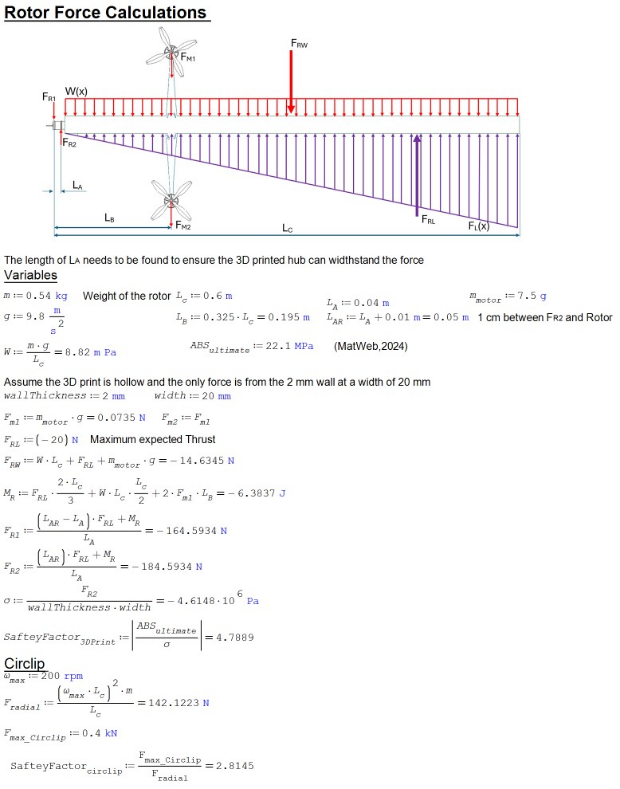
\includegraphics[width =\textwidth, angle=-90]{figs/Design/Rotor/Calcs_3D_Hub_Quality.png}
    % \caption[Segmented blade]{Diagram showing the blade split into segments \citep{blade_element_theory_2024}}
    % \label{fig: blade_segments}
\end{figure}
\begin{figure}[H]
    \centering
    \includegraphics[width =\textwidth]{figs/Design/Rotor/Calcs_Circlip.png}
    % \caption[Segmented blade]{Diagram showing the blade split into segments \citep{blade_element_theory_2024}}
    % \label{fig: blade_segments}
\end{figure}
\begin{landscape}
\includepdf[
    pages=-,
    angle=90,
% Adjust the scale factor to fit the content on the page
]{Appendix Documents/Exploded VIew and Assmebly.pdf}
\end{landscape}


\backmatter%----------------------------------------------------------

\end{document}   

